%!TEX root = ../main.tex
\chapter{Equazione di Laplace-Poisson}

\begin{definition}
    [Equazione di Poisson] Si definisce
    \begin{equation*}
        \boxed{-\Delta u=f} \ \ \text{in} \ \Omega \ \text{dominio limitato in} \ \mathbb{R}^{n}
    \end{equation*}
\end{definition}
da dove viene fuori?
\begin{itemize}
    \item Temperatura a regime stazionario $u_{t}=0$ con $D=1$ dell'equazione del calore.
    \item $\mathbf{E}$ campo elettrostatico generato da una distribuzione di carica $\rho $ in $\Omega \subset \mathbb{R}^{3}$ in unità $Mks$:
          \begin{equation*}
              \mathrm{div}\mathbf{E} =\frac{4\pi \rho }{\varepsilon }
          \end{equation*}

          $\varepsilon $ costante dielettrica.

          Se il campo è conservativo esiste uno scalare $u$, detto potenziale elettrostatico, tale che $\nabla u=-\mathbf{E}$ allora
          \begin{equation*}
              \mathrm{div}\mathbf{E} =-\mathrm{div}(\nabla u) =-\Delta u=\frac{4\pi \rho }{\varepsilon }
          \end{equation*}

          In assenza di cariche $\rho =0$ e quindi il potenziale è armonico $\Delta u=0$.
    \item Le parti reali e immaginarie di una funzione olomorfa sono armoniche. Poiché per esempio le funzioni al variare di $m\in \mathbb{N}$

          \begin{equation*}
              z^{m} =\rho ^{m}(\cos m\vartheta +i\sin m\vartheta)
          \end{equation*}

          sono olomorfe in $\mathbb{C}$, di conseguenza le funzioni

          \begin{equation*}
              \begin{cases}
                  u(\rho,\vartheta) =\rho ^{m}\cos m\vartheta \\
                  v(\rho,\vartheta) =\rho ^{m}\sin m\vartheta
              \end{cases}
          \end{equation*}

          sono armoniche. Tra esse per esempio
          \begin{equation*}
              m=2,\ \ z^{2} =\left(x^{2} -y^{2}\right) +ixy\ \ \Rightarrow \ \ \begin{cases}
                  u=x^{2} -y^{2} \\
                  v=xy
              \end{cases}
          \end{equation*}
\end{itemize}
\section{Tipici problemi al bordo}

Sono le condizioni che troviamo nell'equazione del calore nella parte laterale
\begin{itemize}
    \item \textbf{Dirichlet} $u=g$ su $\partial \Omega $
    \item \textbf{Neumann} $\partial _{\nuu } u=h$ su $\partial \Omega $
    \item \textbf{Robin} $\partial _{\nuu } u+\alpha u=h$, con $\alpha  >0$
    \item miste
\end{itemize}
\LezioneS{16/03/2021}

\begin{theorem}[Unicità]
    Sia $\Omega \subset \mathbb{R}^{n}$ un dominio \textbf{limitato} regolare. Allora esiste al più una funzione $u$ di classe $C^{2}(\Omega) \cap C^{1}(\overline{\Omega })$ soluzione di $-\Delta u=f$ in $\Omega $ con condizioni di Dirichlet o Robin. Nel caso di Neumann, due soluzioni differiscono per una costante.
\end{theorem}
\begin{dimostrazione}
    Siano $u$ e $v$ soluzioni di uno dei problemi indicati con lo stesso dato al bordo $g$. Sia $w=u-v$, allora $w$ è armonica in $\Omega $
    \begin{equation*}
        \Delta w=\Delta u-\Delta v=-f+f=0
    \end{equation*}
    con dato al bordo $g=0$. Moltiplicando per $w$ e integrando su $\Omega $
    \begin{equation*}
        \int _{\Omega } w\Delta w=0
    \end{equation*}
    Da cui, utilizzando l'identità di Green \eqref{eq:id-green}
    \begin{equation*}
        -\int _{\Omega }| \nabla w| ^{2} +\int _{\partial \Omega } w\partial _{\nuu} w\dsig =0\ \ \Rightarrow \ \ \int _{\Omega }| \nabla w| ^{2} =\int _{\partial \Omega } w\partial _{\nuu} w\dsig
    \end{equation*}
    Ora analizziamo nello specifico i tre possibili casi:
    \begin{itemize}
        \item \textbf{Dirichlet}
              \begin{equation*}
                  w=0\ \text{su} \ \partial \Omega \ \ \Rightarrow \ \ \int _{\Omega }| \nabla w| ^{2} =0\ \ \Rightarrow \ \ \nabla w=0\ \text{in} \ \mathrm{\Omega } \ \ \Rightarrow \ \ w=\text{cost. in} \ \Omega
              \end{equation*}

              Ma dato che $w=0$ su $\displaystyle \partial \Omega $ ed essendo $\displaystyle C^{1}$ fino al bordo, la costante deve essere $0$, da cui $\displaystyle w\equiv 0$.
        \item \textbf{Robin}
              \begin{equation*}
                  \partial_{\nuu} w=-\alpha w\ \text{su} \ \partial \Omega \ \ \Rightarrow \ \ \int _{\Omega }| \nabla w| ^{2} =-\alpha \int _{\partial \Omega } w^{2} \dsig \leq 0
              \end{equation*}

              ma essendo il primo integrale $\displaystyle \geq 0$, allora deve essere nullo come prima:
              \begin{equation*}
                  \int _{\Omega }| \nabla w| ^{2} =0\ \ \Rightarrow \ \ \nabla w=0\ \text{in} \ \mathrm{\Omega } \ \ \Rightarrow \ \ w=\text{cost. in} \ \Omega
              \end{equation*}

              Ma dato che è costante, la derivata normale sul bordo è nulla $\displaystyle \partial_{\nuu} w=0=-\alpha w$, quindi $w=0$ sul bordo e, come prima, essendo $\displaystyle C^{1}$ fino al bordo, la costante è nulla, da cui $\displaystyle w\equiv 0$.
        \item \textbf{Neumann}
              \begin{equation*}
                  \partial_{\nuu} w=0\ \text{su} \ \partial \Omega \ \ \Rightarrow \ \ \int _{\Omega }| \nabla w| ^{2} =0\ \ \Rightarrow \ \ \nabla w=0\ \text{in} \ \mathrm{\Omega } \ \ \Rightarrow \ \ w=\text{cost. in} \ \Omega
              \end{equation*}

              Non posso fare alcuna affermazione aggiuntiva.
    \end{itemize}
\end{dimostrazione}
Nel caso Neumann non vale l'unicità, ma in generale non vale neanche l'esistenza, infatti da
\begin{equation*}
    -\Delta u=f,\ \partial _{\nuu} u=g\ \text{su} \ \partial \Omega
\end{equation*}
integrando su $\displaystyle \Omega $ si trova
\begin{equation*}
    -\int _{\Omega } \Delta u=\int _{\Omega } f
\end{equation*}
e applicando il teorema di Gauss \eqref{eq:id-green-v1}
\begin{equation*}
    -\int _{\partial \Omega } \partial_{\nuu} u\dsig =\int _{\Omega } f
\end{equation*}
Abbiamo trovato una \textbf{condizione necessaria per la risolubilità del problema di Neumann}:
\begin{equation}
    \boxed{\int _{\Omega } f\dxx+\int _{\partial \Omega } g\dsig =0}
\end{equation}
Per esempio:
\begin{equation*}
    \begin{cases}
        -\Delta u=1          & \text{in} \ \Omega \\
        \partial _{\nuu} u=0 &
    \end{cases}
\end{equation*}
non ha soluzione! La condizione necessaria che abbiamo trovato infatti darebbe
\begin{equation*}
    \int _{\Omega } 1=0
\end{equation*}
\section{Funzioni armoniche nel discreto}

Per esaminare le proprietà delle funzioni armoniche torniamo ad esplorare il legame tra modelli discreti e continui, probabilistici e deterministici. Ritorniamo alla passeggiata aleatoria, lavorando questa volta in dimensione $n=2$. Allora detti $h >0$ passo spaziale, e $\displaystyle \tau  >0$ passo temporale, introduciamo $\displaystyle h\mathbb{Z}^{2}$ il reticolo dei punti
\begin{equation*}
    \begin{cases}
        \x=(x_{1},x_{2}) &                 \\
        x_{1} =mh        & m\in \mathbb{Z} \\
        x_{2} =nh        & n\in \mathbb{Z}
    \end{cases}
\end{equation*}
La particella si muove in ciascuna delle quattro direzioni con probabilità identica $1/4$, e i versori degli assi $\displaystyle x_{1},x_{2}$ sono rispettivamente $\displaystyle \mathbf{e}_{1},\mathbf{e}_{2}$.

Sia $\displaystyle p(\x,t) =p(x_{1},x_{2},t)$ la probabilità di trovare la particella nel punto $\x$ al tempo $t$. Come nella precedente passeggiata cerchiamo di ricavare un'equazione alle differenze finite per $p$ col teorema delle probabilità totali.
\begin{equation*}
    p(x_{1},x_{2},t+\tau) =\frac{1}{4}\{p(\x-h\mathbf{e}_{1},t) +p(\x+h\mathbf{e}_{1},t) +p(\x-h\mathbf{e}_{2},t) +p(\x+h\mathbf{e}_{2},t)\}
\end{equation*}
Quella che troviamo è esattamente la media aritmetica dei valori di $p(\cdotp,t)$ nei punti dell'intorno discreto di $\x$ di raggio $h$.

Trascurando per ora il tempo, definisco l'operatore di media su una generica funzione $u=u(\x),\x\in h\mathbb{Z}^{2}$
\begin{equation*}
    M_{h} u(\x) =\frac{1}{4}\sum _{| \x-\y| =h} u(\y)
\end{equation*}
In questo modo posso riscrivere l'equazione alle differenze sfruttando l'operatore
\begin{equation*}
    p(x_{1},x_{2},t+\tau) =M_{h} p(\x,t)
\end{equation*}
Sviluppando fino al secondo ordine con Taylor e elidendo opportunamente i termini:
\begin{equation*}
    M_{h} u(\x) =\frac{1}{4}\bigg[4u(\x) +\underbrace{h^{2} u_{x_{1} x_{1}}(\x) +h^{2} u_{x_{2} x_{2}}(\x)}_{h^{2} \Delta u(\x)}\bigg] +o\left(h^{2}\right)
\end{equation*}
passando al limite:
\begin{equation*}
    \lim _{h\rightarrow 0}\frac{M_{h} u(\x) -u(\x)}{h^{2}} =\frac{1}{4} \Delta u(\x)
\end{equation*}
In base a questo risultato è coerente definire il \textbf{laplaciano discreto}
\begin{equation}
    \Delta ^{*}_{h} u(\x) =\frac{4}{h^{2}}(M_{h} u(\x) -u(\x))
\end{equation}
Se $\displaystyle \Delta ^{*}_{h} u=0$ (ovvero se in ogni punto $\x$ la funzione coincide con la media dei propri valori nei punti dell'intorno discreto di $\x$ di raggio $h$) la funzione verrà chiamata \textbf{d-armonica} (dove `d' sta per discreto).

Cerchiamo ora di definire il problema di Dirichlet discreto nel reticolo: per farlo servono prima delle nozioni di topologia discreta.

Sia $\displaystyle A \subset h\mathbb{Z}^{2}$. Diciamo che $\x\in A$ è
\begin{itemize}
    \item \textbf{interno} ad $A$ se il suo intorno discreto di raggio $h$ è contenuto in $A$;
    \item \textbf{punto di frontiera} se non è interno ad $A$ ma il suo intorno discreto di raggio $h$ contiene almeno un punto interno;
    \item \textbf{isolato} se non è interno o di frontiera.
\end{itemize}

$A$ è detto \textbf{connesso} se non ha punti isolati e $\displaystyle \forall x_{0},x_{1} \in A\ x_{0},x_{1}$ possono essere collegati da un cammino discreto contenuto interamente in $A$

%\fg[Esempio di dominio connesso di $\displaystyle h\mathbb{Z}^{2}$]{0.4}{laplace-dominio-connesso-discreto}

\begin{figure}[htpb]
    \centering

    \tikzset{every picture/.style={line width=0.75pt}} %set default line width to 0.75pt        

    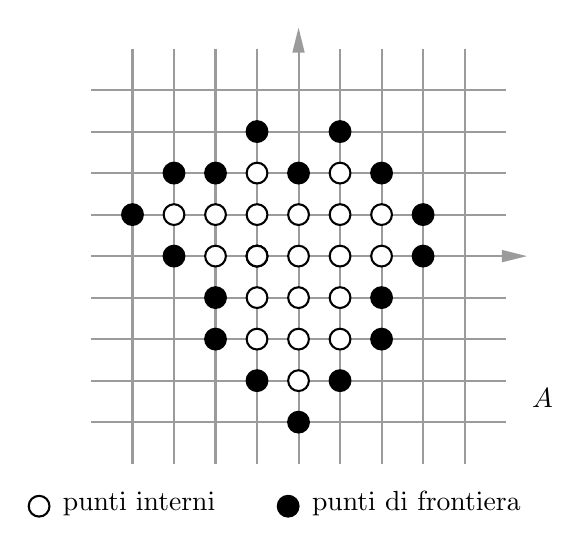
\begin{tikzpicture}[x=0.75pt,y=0.75pt,yscale=-1,xscale=1]
        %uncomment if require: \path (0,262); %set diagram left start at 0, and has height of 262

        %Straight Lines [id:da5353510414709739] 
        \draw [color={rgb, 255:red, 155; green, 155; blue, 155 }  ,draw opacity=1 ]   (180,20) -- (180,220) ;
        %Straight Lines [id:da15467882974727698] 
        \draw [color={rgb, 255:red, 155; green, 155; blue, 155 }  ,draw opacity=1 ]   (200,20) -- (200,220) ;
        %Straight Lines [id:da14275801539205402] 
        \draw [color={rgb, 255:red, 155; green, 155; blue, 155 }  ,draw opacity=1 ]   (220,20) -- (220,220) ;
        %Straight Lines [id:da9190441177768864] 
        \draw [color={rgb, 255:red, 155; green, 155; blue, 155 }  ,draw opacity=1 ]   (240,20) -- (240,220) ;
        %Straight Lines [id:da9212486743534622] 
        \draw [color={rgb, 255:red, 155; green, 155; blue, 155 }  ,draw opacity=1 ]   (260,12) -- (260,220) ;
        \draw [shift={(260,10)}, rotate = 90] [fill={rgb, 255:red, 155; green, 155; blue, 155 }  ,fill opacity=1 ][line width=0.08]  [draw opacity=0] (12,-3) -- (0,0) -- (12,3) -- cycle    ;
        %Straight Lines [id:da43726115644826513] 
        \draw [color={rgb, 255:red, 155; green, 155; blue, 155 }  ,draw opacity=1 ]   (280,20) -- (280,220) ;
        %Straight Lines [id:da19991060674463945] 
        \draw [color={rgb, 255:red, 155; green, 155; blue, 155 }  ,draw opacity=1 ]   (300,20) -- (300,220) ;
        %Straight Lines [id:da48136836452011034] 
        \draw [color={rgb, 255:red, 155; green, 155; blue, 155 }  ,draw opacity=1 ]   (320,20) -- (320,220) ;
        %Straight Lines [id:da8368298047164227] 
        \draw [color={rgb, 255:red, 155; green, 155; blue, 155 }  ,draw opacity=1 ]   (340,20) -- (340,220) ;
        %Straight Lines [id:da06573336765433746] 
        \draw [color={rgb, 255:red, 155; green, 155; blue, 155 }  ,draw opacity=1 ]   (360,40) -- (160,40) ;
        %Straight Lines [id:da12417886977326842] 
        \draw [color={rgb, 255:red, 155; green, 155; blue, 155 }  ,draw opacity=1 ]   (360,60) -- (160,60) ;
        %Straight Lines [id:da11668682972776145] 
        \draw [color={rgb, 255:red, 155; green, 155; blue, 155 }  ,draw opacity=1 ]   (360,80) -- (160,80) ;
        %Straight Lines [id:da7460484192271928] 
        \draw [color={rgb, 255:red, 155; green, 155; blue, 155 }  ,draw opacity=1 ]   (360,100) -- (160,100) ;
        %Straight Lines [id:da4545379688479392] 
        \draw [color={rgb, 255:red, 155; green, 155; blue, 155 }  ,draw opacity=1 ]   (368,120) -- (160,120) ;
        \draw [shift={(370,120)}, rotate = 180] [fill={rgb, 255:red, 155; green, 155; blue, 155 }  ,fill opacity=1 ][line width=0.08]  [draw opacity=0] (12,-3) -- (0,0) -- (12,3) -- cycle    ;
        %Straight Lines [id:da5910363634754043] 
        \draw [color={rgb, 255:red, 155; green, 155; blue, 155 }  ,draw opacity=1 ]   (360,140) -- (160,140) ;
        %Straight Lines [id:da19061706395319145] 
        \draw [color={rgb, 255:red, 155; green, 155; blue, 155 }  ,draw opacity=1 ]   (360,160) -- (160,160) ;
        %Straight Lines [id:da5126660041208353] 
        \draw [color={rgb, 255:red, 155; green, 155; blue, 155 }  ,draw opacity=1 ]   (360,180) -- (160,180) ;
        %Straight Lines [id:da8050524582611216] 
        \draw [color={rgb, 255:red, 155; green, 155; blue, 155 }  ,draw opacity=1 ]   (360,200) -- (160,200) ;
        %Shape: Circle [id:dp9237465481521829] 
        \draw  [fill={rgb, 255:red, 255; green, 255; blue, 255 }  ,fill opacity=1 ] (235,120) .. controls (235,117.24) and (237.24,115) .. (240,115) .. controls (242.76,115) and (245,117.24) .. (245,120) .. controls (245,122.76) and (242.76,125) .. (240,125) .. controls (237.24,125) and (235,122.76) .. (235,120) -- cycle ;
        %Shape: Circle [id:dp7847752425258692] 
        \draw  [fill={rgb, 255:red, 255; green, 255; blue, 255 }  ,fill opacity=1 ] (235,120) .. controls (235,117.24) and (237.24,115) .. (240,115) .. controls (242.76,115) and (245,117.24) .. (245,120) .. controls (245,122.76) and (242.76,125) .. (240,125) .. controls (237.24,125) and (235,122.76) .. (235,120) -- cycle ;
        %Shape: Circle [id:dp6482789236621291] 
        \draw  [fill={rgb, 255:red, 255; green, 255; blue, 255 }  ,fill opacity=1 ] (235,120) .. controls (235,117.24) and (237.24,115) .. (240,115) .. controls (242.76,115) and (245,117.24) .. (245,120) .. controls (245,122.76) and (242.76,125) .. (240,125) .. controls (237.24,125) and (235,122.76) .. (235,120) -- cycle ;
        %Shape: Circle [id:dp11376700055154343] 
        \draw  [fill={rgb, 255:red, 255; green, 255; blue, 255 }  ,fill opacity=1 ] (235,140) .. controls (235,137.24) and (237.24,135) .. (240,135) .. controls (242.76,135) and (245,137.24) .. (245,140) .. controls (245,142.76) and (242.76,145) .. (240,145) .. controls (237.24,145) and (235,142.76) .. (235,140) -- cycle ;
        %Shape: Circle [id:dp5725526937019114] 
        \draw  [fill={rgb, 255:red, 255; green, 255; blue, 255 }  ,fill opacity=1 ] (255,160) .. controls (255,157.24) and (257.24,155) .. (260,155) .. controls (262.76,155) and (265,157.24) .. (265,160) .. controls (265,162.76) and (262.76,165) .. (260,165) .. controls (257.24,165) and (255,162.76) .. (255,160) -- cycle ;
        %Shape: Circle [id:dp029554016948183826] 
        \draw  [fill={rgb, 255:red, 255; green, 255; blue, 255 }  ,fill opacity=1 ] (275,160) .. controls (275,157.24) and (277.24,155) .. (280,155) .. controls (282.76,155) and (285,157.24) .. (285,160) .. controls (285,162.76) and (282.76,165) .. (280,165) .. controls (277.24,165) and (275,162.76) .. (275,160) -- cycle ;
        %Shape: Circle [id:dp8343641165060725] 
        \draw  [fill={rgb, 255:red, 255; green, 255; blue, 255 }  ,fill opacity=1 ] (275,140) .. controls (275,137.24) and (277.24,135) .. (280,135) .. controls (282.76,135) and (285,137.24) .. (285,140) .. controls (285,142.76) and (282.76,145) .. (280,145) .. controls (277.24,145) and (275,142.76) .. (275,140) -- cycle ;
        %Shape: Circle [id:dp9185555874023956] 
        \draw  [fill={rgb, 255:red, 255; green, 255; blue, 255 }  ,fill opacity=1 ] (255,140) .. controls (255,137.24) and (257.24,135) .. (260,135) .. controls (262.76,135) and (265,137.24) .. (265,140) .. controls (265,142.76) and (262.76,145) .. (260,145) .. controls (257.24,145) and (255,142.76) .. (255,140) -- cycle ;
        %Shape: Circle [id:dp8704989683526148] 
        \draw  [fill={rgb, 255:red, 255; green, 255; blue, 255 }  ,fill opacity=1 ] (255,120) .. controls (255,117.24) and (257.24,115) .. (260,115) .. controls (262.76,115) and (265,117.24) .. (265,120) .. controls (265,122.76) and (262.76,125) .. (260,125) .. controls (257.24,125) and (255,122.76) .. (255,120) -- cycle ;
        %Shape: Circle [id:dp4620932814385901] 
        \draw  [fill={rgb, 255:red, 255; green, 255; blue, 255 }  ,fill opacity=1 ] (295,120) .. controls (295,117.24) and (297.24,115) .. (300,115) .. controls (302.76,115) and (305,117.24) .. (305,120) .. controls (305,122.76) and (302.76,125) .. (300,125) .. controls (297.24,125) and (295,122.76) .. (295,120) -- cycle ;
        %Shape: Circle [id:dp5458808109037241] 
        \draw  [fill={rgb, 255:red, 255; green, 255; blue, 255 }  ,fill opacity=1 ] (275,120) .. controls (275,117.24) and (277.24,115) .. (280,115) .. controls (282.76,115) and (285,117.24) .. (285,120) .. controls (285,122.76) and (282.76,125) .. (280,125) .. controls (277.24,125) and (275,122.76) .. (275,120) -- cycle ;
        %Shape: Circle [id:dp14605679202031863] 
        \draw  [fill={rgb, 255:red, 255; green, 255; blue, 255 }  ,fill opacity=1 ] (255,100) .. controls (255,97.24) and (257.24,95) .. (260,95) .. controls (262.76,95) and (265,97.24) .. (265,100) .. controls (265,102.76) and (262.76,105) .. (260,105) .. controls (257.24,105) and (255,102.76) .. (255,100) -- cycle ;
        %Shape: Circle [id:dp21367266026133613] 
        \draw  [fill={rgb, 255:red, 255; green, 255; blue, 255 }  ,fill opacity=1 ] (295,100) .. controls (295,97.24) and (297.24,95) .. (300,95) .. controls (302.76,95) and (305,97.24) .. (305,100) .. controls (305,102.76) and (302.76,105) .. (300,105) .. controls (297.24,105) and (295,102.76) .. (295,100) -- cycle ;
        %Shape: Circle [id:dp45695822274778064] 
        \draw  [fill={rgb, 255:red, 255; green, 255; blue, 255 }  ,fill opacity=1 ] (275,100) .. controls (275,97.24) and (277.24,95) .. (280,95) .. controls (282.76,95) and (285,97.24) .. (285,100) .. controls (285,102.76) and (282.76,105) .. (280,105) .. controls (277.24,105) and (275,102.76) .. (275,100) -- cycle ;
        %Shape: Circle [id:dp3024697868068069] 
        \draw  [fill={rgb, 255:red, 255; green, 255; blue, 255 }  ,fill opacity=1 ] (195,100) .. controls (195,97.24) and (197.24,95) .. (200,95) .. controls (202.76,95) and (205,97.24) .. (205,100) .. controls (205,102.76) and (202.76,105) .. (200,105) .. controls (197.24,105) and (195,102.76) .. (195,100) -- cycle ;
        %Shape: Circle [id:dp31677911941011283] 
        \draw  [fill={rgb, 255:red, 255; green, 255; blue, 255 }  ,fill opacity=1 ] (235,100) .. controls (235,97.24) and (237.24,95) .. (240,95) .. controls (242.76,95) and (245,97.24) .. (245,100) .. controls (245,102.76) and (242.76,105) .. (240,105) .. controls (237.24,105) and (235,102.76) .. (235,100) -- cycle ;
        %Shape: Circle [id:dp42672114879554734] 
        \draw  [fill={rgb, 255:red, 255; green, 255; blue, 255 }  ,fill opacity=1 ] (215,100) .. controls (215,97.24) and (217.24,95) .. (220,95) .. controls (222.76,95) and (225,97.24) .. (225,100) .. controls (225,102.76) and (222.76,105) .. (220,105) .. controls (217.24,105) and (215,102.76) .. (215,100) -- cycle ;
        %Shape: Circle [id:dp9034839574506011] 
        \draw  [fill={rgb, 255:red, 255; green, 255; blue, 255 }  ,fill opacity=1 ] (255,180) .. controls (255,177.24) and (257.24,175) .. (260,175) .. controls (262.76,175) and (265,177.24) .. (265,180) .. controls (265,182.76) and (262.76,185) .. (260,185) .. controls (257.24,185) and (255,182.76) .. (255,180) -- cycle ;
        %Shape: Circle [id:dp6014090171941286] 
        \draw  [fill={rgb, 255:red, 255; green, 255; blue, 255 }  ,fill opacity=1 ] (235,160) .. controls (235,157.24) and (237.24,155) .. (240,155) .. controls (242.76,155) and (245,157.24) .. (245,160) .. controls (245,162.76) and (242.76,165) .. (240,165) .. controls (237.24,165) and (235,162.76) .. (235,160) -- cycle ;
        %Shape: Circle [id:dp8156729691931675] 
        \draw  [fill={rgb, 255:red, 255; green, 255; blue, 255 }  ,fill opacity=1 ] (235,80) .. controls (235,77.24) and (237.24,75) .. (240,75) .. controls (242.76,75) and (245,77.24) .. (245,80) .. controls (245,82.76) and (242.76,85) .. (240,85) .. controls (237.24,85) and (235,82.76) .. (235,80) -- cycle ;
        %Shape: Circle [id:dp7221806604841374] 
        \draw  [fill={rgb, 255:red, 255; green, 255; blue, 255 }  ,fill opacity=1 ] (275,80) .. controls (275,77.24) and (277.24,75) .. (280,75) .. controls (282.76,75) and (285,77.24) .. (285,80) .. controls (285,82.76) and (282.76,85) .. (280,85) .. controls (277.24,85) and (275,82.76) .. (275,80) -- cycle ;
        %Shape: Circle [id:dp29957969253770766] 
        \draw  [fill={rgb, 255:red, 255; green, 255; blue, 255 }  ,fill opacity=1 ] (215,120) .. controls (215,117.24) and (217.24,115) .. (220,115) .. controls (222.76,115) and (225,117.24) .. (225,120) .. controls (225,122.76) and (222.76,125) .. (220,125) .. controls (217.24,125) and (215,122.76) .. (215,120) -- cycle ;
        %Shape: Circle [id:dp3998192401066736] 
        \draw  [fill={rgb, 255:red, 0; green, 0; blue, 0 }  ,fill opacity=1 ] (215,80) .. controls (215,77.24) and (217.24,75) .. (220,75) .. controls (222.76,75) and (225,77.24) .. (225,80) .. controls (225,82.76) and (222.76,85) .. (220,85) .. controls (217.24,85) and (215,82.76) .. (215,80) -- cycle ;
        %Shape: Circle [id:dp2925972276802524] 
        \draw  [fill={rgb, 255:red, 0; green, 0; blue, 0 }  ,fill opacity=1 ] (235,60) .. controls (235,57.24) and (237.24,55) .. (240,55) .. controls (242.76,55) and (245,57.24) .. (245,60) .. controls (245,62.76) and (242.76,65) .. (240,65) .. controls (237.24,65) and (235,62.76) .. (235,60) -- cycle ;
        %Shape: Circle [id:dp9941835548336988] 
        \draw  [fill={rgb, 255:red, 0; green, 0; blue, 0 }  ,fill opacity=1 ] (255,80) .. controls (255,77.24) and (257.24,75) .. (260,75) .. controls (262.76,75) and (265,77.24) .. (265,80) .. controls (265,82.76) and (262.76,85) .. (260,85) .. controls (257.24,85) and (255,82.76) .. (255,80) -- cycle ;
        %Shape: Circle [id:dp8074654402195234] 
        \draw  [fill={rgb, 255:red, 0; green, 0; blue, 0 }  ,fill opacity=1 ] (275,60) .. controls (275,57.24) and (277.24,55) .. (280,55) .. controls (282.76,55) and (285,57.24) .. (285,60) .. controls (285,62.76) and (282.76,65) .. (280,65) .. controls (277.24,65) and (275,62.76) .. (275,60) -- cycle ;
        %Shape: Circle [id:dp4128023300953496] 
        \draw  [fill={rgb, 255:red, 0; green, 0; blue, 0 }  ,fill opacity=1 ] (295,80) .. controls (295,77.24) and (297.24,75) .. (300,75) .. controls (302.76,75) and (305,77.24) .. (305,80) .. controls (305,82.76) and (302.76,85) .. (300,85) .. controls (297.24,85) and (295,82.76) .. (295,80) -- cycle ;
        %Shape: Circle [id:dp6066919254816971] 
        \draw  [fill={rgb, 255:red, 0; green, 0; blue, 0 }  ,fill opacity=1 ] (315,100) .. controls (315,97.24) and (317.24,95) .. (320,95) .. controls (322.76,95) and (325,97.24) .. (325,100) .. controls (325,102.76) and (322.76,105) .. (320,105) .. controls (317.24,105) and (315,102.76) .. (315,100) -- cycle ;
        %Shape: Circle [id:dp6011523494863908] 
        \draw  [fill={rgb, 255:red, 0; green, 0; blue, 0 }  ,fill opacity=1 ] (315,120) .. controls (315,117.24) and (317.24,115) .. (320,115) .. controls (322.76,115) and (325,117.24) .. (325,120) .. controls (325,122.76) and (322.76,125) .. (320,125) .. controls (317.24,125) and (315,122.76) .. (315,120) -- cycle ;
        %Shape: Circle [id:dp7625040461436632] 
        \draw  [fill={rgb, 255:red, 0; green, 0; blue, 0 }  ,fill opacity=1 ] (295,140) .. controls (295,137.24) and (297.24,135) .. (300,135) .. controls (302.76,135) and (305,137.24) .. (305,140) .. controls (305,142.76) and (302.76,145) .. (300,145) .. controls (297.24,145) and (295,142.76) .. (295,140) -- cycle ;
        %Shape: Circle [id:dp9186800386536049] 
        \draw  [fill={rgb, 255:red, 0; green, 0; blue, 0 }  ,fill opacity=1 ] (295,160) .. controls (295,157.24) and (297.24,155) .. (300,155) .. controls (302.76,155) and (305,157.24) .. (305,160) .. controls (305,162.76) and (302.76,165) .. (300,165) .. controls (297.24,165) and (295,162.76) .. (295,160) -- cycle ;
        %Shape: Circle [id:dp4307940010263418] 
        \draw  [fill={rgb, 255:red, 0; green, 0; blue, 0 }  ,fill opacity=1 ] (275,180) .. controls (275,177.24) and (277.24,175) .. (280,175) .. controls (282.76,175) and (285,177.24) .. (285,180) .. controls (285,182.76) and (282.76,185) .. (280,185) .. controls (277.24,185) and (275,182.76) .. (275,180) -- cycle ;
        %Shape: Circle [id:dp6330806171043668] 
        \draw  [fill={rgb, 255:red, 0; green, 0; blue, 0 }  ,fill opacity=1 ] (255,200) .. controls (255,197.24) and (257.24,195) .. (260,195) .. controls (262.76,195) and (265,197.24) .. (265,200) .. controls (265,202.76) and (262.76,205) .. (260,205) .. controls (257.24,205) and (255,202.76) .. (255,200) -- cycle ;
        %Shape: Circle [id:dp3067866836234143] 
        \draw  [fill={rgb, 255:red, 0; green, 0; blue, 0 }  ,fill opacity=1 ] (235,180) .. controls (235,177.24) and (237.24,175) .. (240,175) .. controls (242.76,175) and (245,177.24) .. (245,180) .. controls (245,182.76) and (242.76,185) .. (240,185) .. controls (237.24,185) and (235,182.76) .. (235,180) -- cycle ;
        %Shape: Circle [id:dp2975156996133277] 
        \draw  [fill={rgb, 255:red, 0; green, 0; blue, 0 }  ,fill opacity=1 ] (215,160) .. controls (215,157.24) and (217.24,155) .. (220,155) .. controls (222.76,155) and (225,157.24) .. (225,160) .. controls (225,162.76) and (222.76,165) .. (220,165) .. controls (217.24,165) and (215,162.76) .. (215,160) -- cycle ;
        %Shape: Circle [id:dp8588996985224986] 
        \draw  [fill={rgb, 255:red, 0; green, 0; blue, 0 }  ,fill opacity=1 ] (215,140) .. controls (215,137.24) and (217.24,135) .. (220,135) .. controls (222.76,135) and (225,137.24) .. (225,140) .. controls (225,142.76) and (222.76,145) .. (220,145) .. controls (217.24,145) and (215,142.76) .. (215,140) -- cycle ;
        %Shape: Circle [id:dp2202127111290677] 
        \draw  [fill={rgb, 255:red, 0; green, 0; blue, 0 }  ,fill opacity=1 ] (195,120) .. controls (195,117.24) and (197.24,115) .. (200,115) .. controls (202.76,115) and (205,117.24) .. (205,120) .. controls (205,122.76) and (202.76,125) .. (200,125) .. controls (197.24,125) and (195,122.76) .. (195,120) -- cycle ;
        %Shape: Circle [id:dp2275971430906929] 
        \draw  [fill={rgb, 255:red, 0; green, 0; blue, 0 }  ,fill opacity=1 ] (175,100) .. controls (175,97.24) and (177.24,95) .. (180,95) .. controls (182.76,95) and (185,97.24) .. (185,100) .. controls (185,102.76) and (182.76,105) .. (180,105) .. controls (177.24,105) and (175,102.76) .. (175,100) -- cycle ;
        %Shape: Circle [id:dp26619674093276013] 
        \draw  [fill={rgb, 255:red, 0; green, 0; blue, 0 }  ,fill opacity=1 ] (195,80) .. controls (195,77.24) and (197.24,75) .. (200,75) .. controls (202.76,75) and (205,77.24) .. (205,80) .. controls (205,82.76) and (202.76,85) .. (200,85) .. controls (197.24,85) and (195,82.76) .. (195,80) -- cycle ;
        %Shape: Circle [id:dp9587969814107671] 
        \draw  [fill={rgb, 255:red, 255; green, 255; blue, 255 }  ,fill opacity=1 ] (130,240.5) .. controls (130,237.74) and (132.24,235.5) .. (135,235.5) .. controls (137.76,235.5) and (140,237.74) .. (140,240.5) .. controls (140,243.26) and (137.76,245.5) .. (135,245.5) .. controls (132.24,245.5) and (130,243.26) .. (130,240.5) -- cycle ;
        %Shape: Circle [id:dp7285056686918892] 
        \draw  [fill={rgb, 255:red, 0; green, 0; blue, 0 }  ,fill opacity=1 ] (250,240.5) .. controls (250,237.74) and (252.24,235.5) .. (255,235.5) .. controls (257.76,235.5) and (260,237.74) .. (260,240.5) .. controls (260,243.26) and (257.76,245.5) .. (255,245.5) .. controls (252.24,245.5) and (250,243.26) .. (250,240.5) -- cycle ;

        % Text Node
        \draw (145,232) node [anchor=north west][inner sep=0.75pt]   [align=left] {punti interni};
        % Text Node
        \draw (265,232) node [anchor=north west][inner sep=0.75pt]   [align=left] {punti di frontiera};
        % Text Node
        \draw (371,182.4) node [anchor=north west][inner sep=0.75pt]    {$A$};

    \end{tikzpicture}
    \caption{Esempio di dominio connesso di $\displaystyle h\mathbb{Z}^{2}$}
\end{figure}
\FloatBarrier

\textbf{Problema di Dirichlet discreto}: sia $A$ dominio limitato e connesso di $\displaystyle h\mathbb{Z}^{2}$, sia $g$ definita su $\displaystyle \partial A$. Determinare $u$, definito su $A$, tale che
\begin{equation}
    \tag{P$_{h,\text{Dirichlet}}$}
    \begin{cases}
        \Delta ^{*}_{h} u=0 & \text{nei punti interni ad} \ A \\
        u=g                 & \text{su} \ \partial A
    \end{cases}
    \label{eq:pb-dirichlet-discreto}
\end{equation}
Proprietà di una soluzione di \eqref{eq:pb-dirichlet-discreto}:
\begin{enumerate}
    \item \textbf{Principio di massimo}. Se $u$ assume massimo o minimo in un punto interno ad $A$, allora $u$ è costante. Infatti
          \begin{figure}[htpb]
              \centering

              \tikzset{every picture/.style={line width=0.75pt}} %set default line width to 0.75pt        

              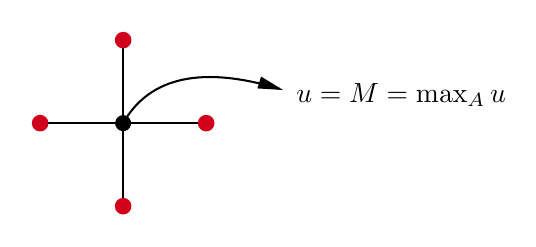
\begin{tikzpicture}[x=0.75pt,y=0.75pt,yscale=-1,xscale=1]
                  %uncomment if require: \path (0,106); %set diagram left start at 0, and has height of 106

                  %Straight Lines [id:da019234409051198664] 
                  \draw    (120,60) -- (200,60) ;
                  %Straight Lines [id:da2169607633909847] 
                  \draw    (160,20) -- (160,100) ;
                  %Shape: Ellipse [id:dp036734699586719044] 
                  \draw  [draw opacity=0][fill={rgb, 255:red, 208; green, 2; blue, 27 }  ,fill opacity=1 ][line width=3]  (156,20) .. controls (156,17.79) and (157.79,16) .. (160,16) .. controls (162.21,16) and (164,17.79) .. (164,20) .. controls (164,22.21) and (162.21,24) .. (160,24) .. controls (157.79,24) and (156,22.21) .. (156,20) -- cycle ;
                  %Curve Lines [id:da06865790719302067] 
                  \draw    (160,60) .. controls (172.81,37.34) and (198.61,32.35) .. (235.32,43.48) ;
                  \draw [shift={(237,44)}, rotate = 197.42000000000002] [fill={rgb, 255:red, 0; green, 0; blue, 0 }  ][line width=0.08]  [draw opacity=0] (12,-3) -- (0,0) -- (12,3) -- cycle    ;
                  \draw [shift={(160,60)}, rotate = 299.48] [color={rgb, 255:red, 0; green, 0; blue, 0 }  ][fill={rgb, 255:red, 0; green, 0; blue, 0 }  ][line width=0.75]      (0, 0) circle [x radius= 3.35, y radius= 3.35]   ;
                  %Shape: Ellipse [id:dp4253248089812065] 
                  \draw  [draw opacity=0][fill={rgb, 255:red, 208; green, 2; blue, 27 }  ,fill opacity=1 ][line width=3]  (196,60) .. controls (196,57.79) and (197.79,56) .. (200,56) .. controls (202.21,56) and (204,57.79) .. (204,60) .. controls (204,62.21) and (202.21,64) .. (200,64) .. controls (197.79,64) and (196,62.21) .. (196,60) -- cycle ;
                  %Shape: Ellipse [id:dp674183510238525] 
                  \draw  [draw opacity=0][fill={rgb, 255:red, 208; green, 2; blue, 27 }  ,fill opacity=1 ][line width=3]  (156,100) .. controls (156,97.79) and (157.79,96) .. (160,96) .. controls (162.21,96) and (164,97.79) .. (164,100) .. controls (164,102.21) and (162.21,104) .. (160,104) .. controls (157.79,104) and (156,102.21) .. (156,100) -- cycle ;
                  %Shape: Ellipse [id:dp7646484647440714] 
                  \draw  [draw opacity=0][fill={rgb, 255:red, 208; green, 2; blue, 27 }  ,fill opacity=1 ][line width=3]  (116,60) .. controls (116,57.79) and (117.79,56) .. (120,56) .. controls (122.21,56) and (124,57.79) .. (124,60) .. controls (124,62.21) and (122.21,64) .. (120,64) .. controls (117.79,64) and (116,62.21) .. (116,60) -- cycle ;

                  % Text Node
                  \draw (242,39.4) node [anchor=north west][inner sep=0.75pt]    {$u=M=\max_{A} u$};

              \end{tikzpicture}
          \end{figure}
          \FloatBarrier
          Se $u=M$ al centro e $u$ è la media dei punti del suo intorno discreto, anch'essi devono essere punti di massimo. Reiterando il ragionamento per ogni altro punto dell'intorno posso propagarlo fino alla frontiera.
    \item $u$ assume massimo e minimo su $\partial A$ (immediata conseguenza del punto 1)\footnote{Se lo assume dentro, è costante e quindi lo assume anche sul bordo. Se lo assume sul bordo... lo assume sul bordo. Ma và?}.
    \item La soluzione di \eqref{eq:pb-dirichlet-discreto} è unica. Infatti se fossero $2$, la differenza $w=v-u$ sarebbe armonica e nulla al bordo, ma essendo il massimo e minimo assunti sul bordo, segue che $w=0$ in tutto il dominio.
\end{enumerate}
Posso risolvere il problema di Dirichlet discreto con metodi probabilistici, tornando alla passeggiata aleatoria.

Interpretiamo $g$ come una sorta di \textbf{guadagno}: se la particella parte da $\x$ e raggiunge la frontiera di $A$ per la prima volta in $\y$ otteniamo un guadagno $g(\y)$. Voglio dimostrare che, qualunque sia il punto di partenza $\x$, la particella raggiunge $\partial A$ con probabilità $1$ e che il valore di $u(\x)$, la soluzione che vogliamo costruire, è il valore atteso del guadagno $g$ rispetto ad un'opportuna distribuzione di probabilità su $\partial A$.

Indichiamo con $\Gamma $ un qualunque sottoinsieme di $\partial A$ e con $P(\x,\Gamma)$ la probabilità che la particella che parte da $\x$ raggiunga per la prima volta la $\partial A$ in un punto $\y\in \Gamma $.

Dobbiamo dimostrare che $P(\x,\partial A) =1\ \forall \x\in A$. Indico con $w_{\Gamma }(\x)$ la funzione che ottengo al variare di $\x$ in $P(\x,\Gamma)$ con $\Gamma $ fissato:
\begin{equation*}
    \x\longmapsto w_{\Gamma }(\x) \equiv P(\x,\Gamma),\ \Gamma \ \text{fissato}
\end{equation*}
Facciamo vedere che è d-armonica nei punti interni ad $A$, cioè che $\Delta ^{*}_{h} w_{\Gamma } =0$. Usando il teorema delle probabilità totali
\begin{equation*}
    w_{\Gamma }(\x) =P(\x,\Gamma) =\frac{1}{4}\sum _{| \x-\y| =h} P(\y,\Gamma) =\frac{1}{4}\sum _{| \x-\y| =h} w_{\Gamma }(\y) =M_{h} w_{\Gamma }(\x)
\end{equation*}
Da cui
\begin{gather*}
    M_{h} w_{\Gamma }(\x) -w_{\Gamma }(\x) =0 \quad \Rightarrow \quad \Delta ^{*}_{h} w_{\Gamma } =\frac{4}{h^{2}}(M_{h} w_{\Gamma }(\x) -w_{\Gamma }(\x)) =0
\end{gather*}
in tutti i punti interni ad $A$!

Quindi:
\begin{align*}
    \x\in \Gamma                    & \Rightarrow P(\x,\Gamma)=1 \\
    \x\in \partial A\setminus\Gamma & \Rightarrow P(\x,\Gamma)=0
\end{align*}
In particolare se $\Gamma =\partial A$, $w_{\partial A}(\x) =P(\x,\partial A)$ è soluzione del problema di Dirichlet discreto con valore 1 sul bordo ($g\equiv 1)$
\begin{equation*}
    \begin{cases}
        \Delta ^{*}_{h} w_{\partial A}(\x) =0 & \x\ \text{interno ad} \ A \\
        w_{\partial A}(\x) =1                 & \x\in \partial A
    \end{cases}
\end{equation*}
Ma anche la funzione $z(\x) \equiv 1$ è d-armonica, con gli stessi valori al bordo e soluzione dello stesso problema di Dirichlet. Poiché per la terza proprietà, la soluzione è unica
\begin{gather*}
    w_{\partial A}(\x) =z(\x) \equiv 1\ \forall \x\in A \quad \Rightarrow \quad w_{\partial A}(\x) =P(\x,\partial A) =1\ \forall \x\in A
\end{gather*}
La probabilità di raggiungere la frontiera di $A$ partendo da un \textbf{qualunque punto interno di} $A$ è uguale a $1$. Se invece prendiamo la funzione
\begin{equation*}
    \Gamma \longmapsto P(\x,\Gamma),\ \x\ \text{fissato}
\end{equation*}
con $P(\x,\partial A) =1$, prendendo $\Gamma _{1},\Gamma _{2} \subset \partial A$, $\Gamma _{1} \cap \Gamma _{2} =\emptyset $
\begin{equation*}
    P(\x,\Gamma _{1} \cup \Gamma _{2}) =P(\x,\Gamma _{1}) +P(\x,\Gamma _{2})
\end{equation*}
è additiva e definisce dunque una misura di probabilità su $\partial A$, $\forall \x\in A$ fissato. Fatti tutti questi passaggi possiamo ora costruire la soluzione $u$.
\begin{theorem}
    Il valore della soluzione $u$ di \eqref{eq:pb-dirichlet-discreto} è il valore atteso dei guadagni $g(\y)$ rispetto alla distribuzione di probabilità $P(\x,\Gamma)$ cioè
    \begin{equation*}
        u(\x) =\sum _{\y\in \partial A} g(\y) P(\x,\{\y\})
    \end{equation*}
\end{theorem}
\begin{dimostrazione} Dimostriamo in due passi.
    \begin{itemize}
        \item Ogni addendo
              \begin{equation*}
                  g(\y) P(\x,\{\y\}) =g(\y) w_{\{\y\}}(\x)
              \end{equation*}
              è d-armonico in $A$, quindi anche $u$ lo è.

        \item Se $\x\in \partial A$, notiamo che
              \begin{equation*}
                  \begin{cases}
                      P(\x,\{\y\}) =1 & \x=\y,     \\
                      P(\x,\{\y\}) =0 & \x\neq \y.
                  \end{cases}
              \end{equation*}
              Nella soluzione in esame
              \begin{equation*}
                  u(\x) =\sum _{\y\in \partial A} g(\y) P(\x,\{\y\})
              \end{equation*}
              per le $\x$ sul bordo, ogni termine nella somma è uguale a $g(\x)$ se $\y=\x$ oppure a zero se $\y\neq \x$ (\textit{accendi e spegni}).
              La condizione al bordo $u(\x) =g(\x)$ è quindi rispettata.
    \end{itemize}
\end{dimostrazione}
\section{Funzioni armoniche}

Sia $\Omega \subseteq \mathbb{R}^{n}$ un dominio, $u$ è armonica in $\Omega $ se $u\in C^{2}(\Omega)$ e $\Delta u=0$ in $\Omega $.

Quando il passo spaziale $h\rightarrow 0$ le funzioni d-armoniche ``diventano'' armoniche: è ragionevole che versioni appropriate delle proprietà per funzioni d-armoniche continuino a valere nel caso continuo. La prima è la proprietà di media.
\subsection{Proprietà di media}

Le funzioni d-armoniche sono definite in termini di proprietà di media, quindi ci aspettiamo che le funzioni armoniche ereditino una proprietà di media del tipo: il valore al centro di ogni sfera $B_{R}(\x) \subset \subset \Omega $\footnote{Questa notazione è equivalente a $\overline{B_{R}}(x) \subset \Omega $, indica che la supeficie della sfera non tocca la frontiera di $\Omega $.} è uguale alla media artimetica dei valori al bordo della sfera $\partial B_{R}$.

Indichiamo con $\omega _{n}$ la misura di $\partial B_{1}$, la superficie della sfera in $n$ dimensioni di raggio $1$. Quindi $w_{n} =| \partial B_{1}| $:
\begin{align*}
    w_{2} & =2\pi                                                   \\
    w_{3} & =4\pi                                                   \\
    w_{n} & =\frac{n\pi ^{n/2}}{\Gamma \left(\frac{n}{2} +1\right)}
\end{align*}
Dove la funzione Gamma di Eulero è definita come
\begin{equation*}
    \Gamma (s) =\int ^{+\infty }_{0} t^{s-1} e^{-t} \dt
\end{equation*}
\begin{theorem}
    \label{thm:armonica-allora-pdm}
    Sia $u$ armonica ($u\in C^{2}(\Omega)$ e $\Delta u=0$) con $\Omega \subset \mathbb{R}^{n}$. Allora per ogni sfera $B_{R}(\x) \subset \subset \Omega $ valgono le seguenti formule:\footnote{Nota che $w_{n} R^{n-1}$ è la misura $| \partial B_{R}(\x)| $, mentre $\frac{w_{n} R^{n}}{n}$ è semplicemente la misura $| B_{R}(\x)| $. I due coefficienti moltiplicativi nelle formule non fanno altro che riscalare rispettivamente per la misura della superficie della sfera e per la misura della sfera stessa: da questo deriva l'interpretazione di ``proprietà di media''.}
    \begin{equation}
        \tag{PDM$_{\text{sup}}$}
        u(\x) =\frac{1}{w_{n} R^{n-1}}\int _{\partial B_{R}(\x)} u(\sigg) \dsig
        \label{eq:lap-prop-media-sup}
    \end{equation}
    \begin{equation}
        \tag{PDM$_{\text{vol}}$}
        u(\x) =\frac{n}{w_{n} R^{n}}\int _{B_{R}(\x)} u(\y) \dyy
        \label{eq:lap-prop-media-vol}
    \end{equation}
\end{theorem}
\begin{dimostrazione}
    Dimostriamo prima la \eqref{eq:lap-prop-media-sup}. Per $0< r< R$ definiamo
    \begin{equation*}
        g(r) =\frac{1}{w_{n} r^{n-1}}\int _{\partial B_{r}(\x)} u(\sigg) \dsig
    \end{equation*}
    Voglio dimostrare che $g(r)$ è costante e quindi che $\displaystyle g'(r) =0$ per $\displaystyle 0< r< R$. Effettuo un cambio di variabili $\displaystyle \sigg '=\frac{\sigg -\x}{r}$, ovvero $\displaystyle \sigg =\x +r\sigg '$, in modo tale che $\displaystyle \sigg '\in \partial B_{1}(\zer)$ e
    \begin{equation*}
        \dsig =r^{n-1} \dsig '
    \end{equation*}
    quest'ultima considerazione si può intuire considerando la seguente figura
    \begin{figure}[H]
        \centering
        \tikzset{every picture/.style={line width=0.75pt}} %set default line width to 0.75pt        

        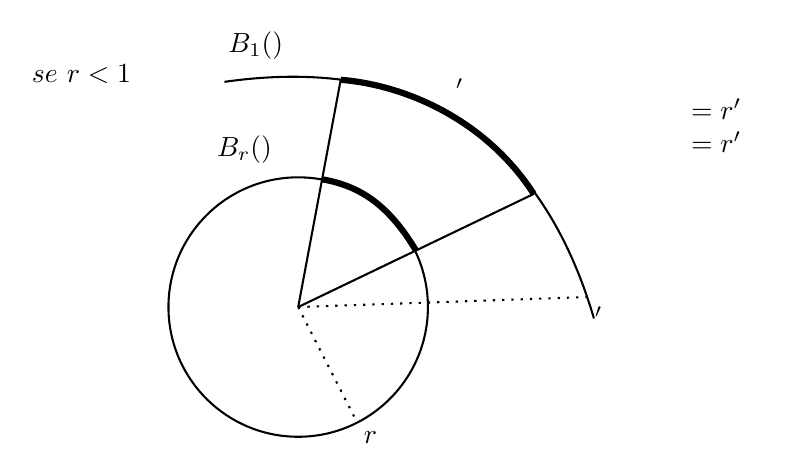
\begin{tikzpicture}[x=0.75pt,y=0.75pt,yscale=-1,xscale=1]
            %uncomment if require: \path (0,225); %set diagram left start at 0, and has height of 225

            %Shape: Circle [id:dp16163150313387842] 
            \draw   (75,152.5) .. controls (75,117.98) and (102.98,90) .. (137.5,90) .. controls (172.02,90) and (200,117.98) .. (200,152.5) .. controls (200,187.02) and (172.02,215) .. (137.5,215) .. controls (102.98,215) and (75,187.02) .. (75,152.5) -- cycle ;
            %Curve Lines [id:da2589776684776446] 
            \draw    (102,44) .. controls (186,32) and (252,63) .. (280,158) ;
            %Straight Lines [id:da7532946855418718] 
            \draw    (137.5,152.5) -- (158,43) ;
            %Straight Lines [id:da8053969796158809] 
            \draw    (137.5,152.5) -- (251,98) ;
            %Straight Lines [id:da30147052897616433] 
            \draw  [dash pattern={on 0.84pt off 2.51pt}]  (137.5,152.5) -- (165.67,207.67) ;
            %Straight Lines [id:da5002817700179074] 
            \draw  [dash pattern={on 0.84pt off 2.51pt}]  (277,147.67) -- (137.5,152.5) ;
            %Curve Lines [id:da48420367449440693] 
            \draw [line width=2.25]    (149.33,91) .. controls (168.33,94.33) and (181.67,104.33) .. (194.25,125.25) ;
            %Curve Lines [id:da6329692248801806] 
            \draw [line width=2.25]    (158,43) .. controls (190.33,45.67) and (228.33,63) .. (251,98) ;

            % Text Node
            \draw (125.33,154.73) node [anchor=north west][inner sep=0.75pt]    {$\zer$};
            % Text Node
            \draw (167.67,211.07) node [anchor=north west][inner sep=0.75pt]    {$r$};
            % Text Node
            \draw (201.33,152.57) node [anchor=north west][inner sep=0.75pt]    {$\sigg$};
            % Text Node
            \draw (279,151.07) node [anchor=north west][inner sep=0.75pt]    {$\sigg '$};
            % Text Node
            \draw (175.33,84.57) node [anchor=north west][inner sep=0.75pt]    {$\dsig$};
            % Text Node
            \draw (212,41.23) node [anchor=north west][inner sep=0.75pt]    {$\dsig '$};
            % Text Node
            \draw (97,68.4) node [anchor=north west][inner sep=0.75pt]    {$B_{r}(\zer)$};
            % Text Node
            \draw (102.33,18.4) node [anchor=north west][inner sep=0.75pt]    {$B_{1}(\x)$};
            % Text Node
            \draw (7.67,34.4) node [anchor=north west][inner sep=0.75pt]    {$\text{se} \ r< 1$};
            % Text Node
            \draw (318.67,49.23) node [anchor=north west][inner sep=0.75pt]    {$ \begin{array}{l}
                        \sigg =r\sigg ' \\
                        \dsig =r\dsig '
                    \end{array}$};
        \end{tikzpicture}
    \end{figure}
    \FloatBarrier

    Il concetto si estende opportunamente a $n$ dimensioni: le lunghezze diventano superfici, poi volumi, ecc.
    \begin{equation*}
        g(r) =\frac{1}{w_{n}\cancel{r^{n-1}}}\int _{\partial B_{1}(\zer)}\cancel{r^{n-1}} u(\x +r\sigg ') \dsig '=\frac{1}{w_{n}}\int _{\partial B_{1}(\zer)} u(\x +r\sigg ') \dsig '
    \end{equation*}
    La regione di integrazione ora non dipende da $r$. Calcoliamo la derivata:
    \begin{equation*}
        g'(r) =\frac{1}{w_{n}}\int _{\partial B_{1}(\zer)}\frac{\de}{\dr} u(\x +r\sigg ') \dsig '=\frac{1}{w_{n}}\int _{\partial B_{1}(\zer)} \nabla u(\x +r\sigg ') \cdotp \sigg '\dsig '
    \end{equation*}
    Sulla sfera $\displaystyle \partial B_{1}(\zer)$, il vettore coincide col vettore normale $\displaystyle \sigg '=\nuu$.
    Poniamo:
    \begin{equation*}
        v(\y)=u(\x+r\y) \quad \Rightarrow \quad \nabla v(\y)=r\nabla u(\x+r\y)\qquad \Delta v(\y)=r^2 \Delta u(\x+r\y)
    \end{equation*}
    Dobbiamo pensare $\x$ come fissato. Usando il teorema della divergenza e ricordando che $u$ è armonica:
    \begin{equation*}
        g'(r) =\frac{1}{w_{n}r}\int _{\partial B_{1}(\zer)} \nabla  v(\sigg') \cdot \sigg' \dsig' =\frac{1}{w_{n}r}\int _{B_{1}(\zer)} \Delta   v(\y) \cdot \y \dyy   =\frac{r}{w_{n}}\int _{B_{1}(\zer)} \Delta u(\x +r\y) \dyy\overset{\Delta u=0}{=} 0.
    \end{equation*}
    Dunque $g$ è costante. Quindi per continuità di $u$:
    \begin{align*}
        g(r) & \xrightarrow{r\rightarrow 0^{+}} u(\x)                                                       \\
        g(r) & \xrightarrow{r\rightarrow R}\frac{1}{w_{n} R^{n-1}}\int _{\partial B_{R}(\x)} u(\sigg) \dsig
    \end{align*}
    Eguagliando i due termini otteniamo la \eqref{eq:lap-prop-media-sup}.

    Per ottenere la \eqref{eq:lap-prop-media-vol} enunciamo ulteriori risultati separatamente per mettere in luce alcuni aspetti.
\end{dimostrazione}

\begin{definition}[PDM]
    Più in generale si dice che una funzione $u\in C(\Omega)$ in $\Omega \subset \mathbb{R}^{n}$ soddisfa la proprietà di media superficiale se vale \eqref{eq:lap-prop-media-sup} e soddisfa la proprietà di media volumentrica se vale \eqref{eq:lap-prop-media-vol}.
\end{definition}
\begin{theorem}
    Se $u\in C(\Omega)$ allora le due \eqref{eq:lap-prop-media-sup} e \eqref{eq:lap-prop-media-vol} sono equivalenti.
\end{theorem}
\begin{dimostrazione}
    Partiamo da
    \begin{equation*}
        u(\x) =\frac{1}{w_{n} r^{n-1}}\int _{\partial Br(\x)} u(\sigg) \dsig
    \end{equation*}
    moltiplichiamo per $r^{n-1}$ e integriamo tra $0$ ed $R$:\footnote{Riordinando gli integrali con fubini sul membro di destra otteniamo una formula di "riduzione per bucce"
        \begin{equation*}
            \int _{B_{R}(\x)} f(y) \dy=\int _{0}^{R}\left(\int _{\partial B_{r}(\x)} f\dsig \right) \dr
        \end{equation*}
    }
    \begin{align*}
        \int _{0}^{R} r^{n-1} u(\x) \dr           & =\frac{1}{w_{n}}\int _{0}^{R} dr\int _{\partial B_{r}(\x)} u(\sigg) \dsig &                 \\
        u(\x)\left[\frac{r^{n}}{n}\right]_{0}^{R} & =\frac{1}{w_{n}}\int _{B_{R}(\x)} u(\y) \dyy                              & \text{(Fubini)} \\
        u(\x)\frac{R^{n}}{n}                      & =\frac{1}{w_{n}}\int _{B_{R}(\x)} u(\y) \dyy                              &
    \end{align*}
    Da cui
    \begin{equation*}
        u(\x) =\frac{n}{w^{n} R^{n}}\int _{B_{R}(\x)} u(\y) \dyy
    \end{equation*}
    Il risultato inverso si ottiene ripercorrendo i passaggi all'indietro.
\end{dimostrazione}
Abbiamo quindi dimostrato che sotto ipotesi più generali, ovvero $u$ solo continua, le due sono equivalenti. È chiaro che sotto ipotesi più strette, $u\in C^{2}$, devono ancora essere equivalenti, pertanto lo sono anche nel contesto del teorema \vref{thm:armonica-allora-pdm}, questo ne conclude la dimostrazione.

Abbiamo dimostrato che se una funzione è armonica allora vale la proprietà di media, ma è vero anche il contrario:
\begin{theorem}
    Sia $\Omega \subset \mathbb{R}^{n}$ un dominio limitato. Se $u\in C(\Omega)$ e ha la proprietà di media in $\Omega $, allora $u\in C^{\infty }(\Omega)$ e $\Delta u=0$ in $\Omega $.
\end{theorem}
Rimarchiamo il fatto che come ipotesi è sufficiente la continuità e la proprietà di media.
\begin{dimostrazione}
    Basta dimostrare che $u\in C^{\infty }(B)$ e $\Delta u=0$ in $B$, dove $B$ è una qualunque sfera contenuta in $\Omega $. Sia dunque $B\subset \subset \Omega $ e sia $v$ la soluzione di
    \begin{equation*}
        \begin{cases}
            \Delta v=0 & \text{in} \ B          \\
            v=u        & \text{su} \ \partial B
        \end{cases}
    \end{equation*}
    $v\in C^{\infty }(B) \cap C(\overline{B})$ perchè soluzione del problema di Poisson\footnote{Vedi il prossimo capitolo su formula di Poisson.}. Anche $v$, essendo armonica in $B$, ha la proprietà di media in $B$. Definisco
    \begin{equation*}
        \ w=u-v
    \end{equation*}
    Anch'essa ha la proprietà della media in $B$, essendo la pdm additiva. Dal teorema \vref{thm:principio-di-massimo-armoniche} segue che $w$ assume massimo e minimo su $\partial B$, ma essendo $w=0$ su $\partial B$, allora
    \begin{equation*}
        w=0\ \text{in} \ \overline{B} \quad \Rightarrow \quad u=v\ \text{in} \ \overline{B}.
    \end{equation*}
\end{dimostrazione}
\subsection{Principio di massimo}

\begin{theorem}[Principio di massimo]
    \label{thm:principio-di-massimo-armoniche}
    Sia $\Omega \subseteq \mathbb{R}^{n}$ e $u\in C(\Omega)$. Se $u$ ha la proprietà della media in $\Omega $, e $u$ assume massimo o minimo in un punto di $\Omega $, allora $u$ è costante. Inoltre, se $\Omega $ è limitato e $u\in C(\overline{\Omega })$ (non costante) allora assume il massimo sul bordo:
    \begin{equation*}
        u(\x) < \max_{\partial \Omega } u,\ u(\x)  >\min_{\partial \Omega } u\ \ \forall \x\in \Omega
    \end{equation*}
\end{theorem}
È implicito che in un dominio illimitato, non essendoci bordo, la soluzione è per forza costante.
\begin{dimostrazione}
    Sia $\mathbf{p}\in \Omega $ punto di minimo
    \begin{equation*}
        m=u(\mathbf{p}) \leq u(\y) \ \forall \y\in \Omega
    \end{equation*}
    Vogliamo dimostrare che $u(x) =m\ \forall x\in \Omega $.

    Sia $\mathbf{q}\in \Omega $ arbitrario. Poiché $\Omega $ è connesso, possiamo trovare una sequenza finita di sfere $B(\x_{j}) \subset \subset \Omega,\ j=0,..,N$ tali che
    \begin{itemize}
        \item $\x_{0} =\mathbf{p},\ x_{N} =\mathbf{q}$
        \item $\x_{j} \in B(\x_{j-1})$
    \end{itemize}
    \fg[Sequenza di cerchi sovrapposti che connettono i punti $\mathbf{p}$ e $\mathbf{q}$]{0.25}{laplace-dim-principio-massimo}
    Per assurdo supponiamo esista $\mathbf{z}\in B(\mathbf{p})$ tale che $u(\mathbf{z})  >m$. Sia $B_{r}(\mathbf{z}) \subset B(\mathbf{p})$

    \begin{figure}[H]
        \centering
        \tikzset{every picture/.style={line width=0.75pt}} %set default line width to 0.75pt        

        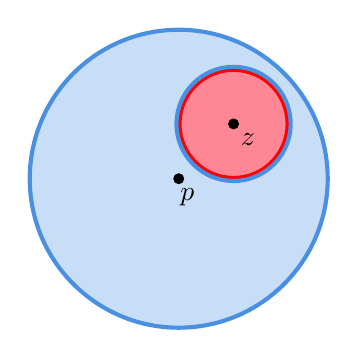
\begin{tikzpicture}[x=0.75pt,y=0.75pt,yscale=-1,xscale=1]
            %uncomment if require: \path (0,152); %set diagram left start at 0, and has height of 152

            %Shape: Circle [id:dp06686904773347901] 
            \draw  [color={rgb, 255:red, 74; green, 144; blue, 226 }  ,draw opacity=1 ][fill={rgb, 255:red, 74; green, 144; blue, 226 }  ,fill opacity=0.3 ][line width=1.5]  (184.83,73.39) .. controls (184.83,33.76) and (216.97,1.62) .. (256.61,1.62) .. controls (296.24,1.62) and (328.38,33.76) .. (328.38,73.39) .. controls (328.38,113.03) and (296.24,145.17) .. (256.61,145.17) .. controls (216.97,145.17) and (184.83,113.03) .. (184.83,73.39) -- cycle ;
            %Shape: Ellipse [id:dp1943751883500897] 
            \draw  [draw opacity=0][fill={rgb, 255:red, 0; green, 0; blue, 0 }  ,fill opacity=1 ][line width=3]  (253.96,73.39) .. controls (253.96,71.94) and (255.15,70.75) .. (256.61,70.75) .. controls (258.06,70.75) and (259.25,71.94) .. (259.25,73.39) .. controls (259.25,74.85) and (258.06,76.04) .. (256.61,76.04) .. controls (255.15,76.04) and (253.96,74.85) .. (253.96,73.39) -- cycle ;
            %Shape: Ellipse [id:dp04152500828404748] 
            \draw  [color={rgb, 255:red, 255; green, 0; blue, 0 }  ,draw opacity=1 ][fill={rgb, 255:red, 255; green, 135; blue, 149 }  ,fill opacity=1 ][line width=1.5]  (256.96,46.98) .. controls (256.96,32.59) and (268.63,20.92) .. (283.02,20.92) .. controls (297.41,20.92) and (309.08,32.59) .. (309.08,46.98) .. controls (309.08,61.37) and (297.41,73.04) .. (283.02,73.04) .. controls (268.63,73.04) and (256.96,61.37) .. (256.96,46.98) -- cycle ;
            %Shape: Ellipse [id:dp09002262431454922] 
            \draw  [draw opacity=0][fill={rgb, 255:red, 0; green, 0; blue, 0 }  ,fill opacity=1 ][line width=3]  (280.38,46.98) .. controls (280.38,45.52) and (281.56,44.34) .. (283.02,44.34) .. controls (284.48,44.34) and (285.66,45.52) .. (285.66,46.98) .. controls (285.66,48.44) and (284.48,49.62) .. (283.02,49.62) .. controls (281.56,49.62) and (280.38,48.44) .. (280.38,46.98) -- cycle ;
            %Shape: Circle [id:dp12636405764113223] 
            \draw  [color={rgb, 255:red, 74; green, 144; blue, 226 }  ,draw opacity=1 ][line width=1.5]  (255.52,46.98) .. controls (255.52,31.79) and (267.83,19.48) .. (283.02,19.48) .. controls (298.21,19.48) and (310.52,31.79) .. (310.52,46.98) .. controls (310.52,62.17) and (298.21,74.48) .. (283.02,74.48) .. controls (267.83,74.48) and (255.52,62.17) .. (255.52,46.98) -- cycle ;

            % Text Node
            \draw (255.96,76.79) node [anchor=north west][inner sep=0.75pt]    {$p$};
            % Text Node
            \draw (285.02,50.38) node [anchor=north west][inner sep=0.75pt]    {$z$};

        \end{tikzpicture}
    \end{figure}
    \FloatBarrier

    Dalla proprietà della media so che
    \begin{equation*}
        m=u(\mathbf{p}) =\frac{1}{| B(\mathbf{p})| }\int _{B(\mathbf{p})} u(\y) \dyy=\frac{1}{| B(\mathbf{p})| }\left[\textcolor[rgb]{0.29,0.56,0.89}{\int _{B(\mathbf{p}) \backslash B_{r}(z)} u(\y) \dyy} +\textcolor[rgb]{0.82,0.01,0.11}{\int _{B_{r}(\mathbf{z})} u(\y) \dyy}\right]
    \end{equation*}
    Sul primo integrale $u(y) \geq m$.

    Sul secondo integrale posso sfruttare ancora la proprietà della media:
    \begin{equation*}
        \int _{B_{r}(\mathbf{z})} u(\y) \dyy=u(\mathbf{z})| B_{r(\mathbf{z})}|  >m| B_{r}(\mathbf{z})|
    \end{equation*}
    Ma allora ottengo una contraddizione
    \begin{equation*}
        m >\frac{1}{| B(\mathbf{p})| }\{m| B(\mathbf{p}) \backslash B_{r}(\mathbf{z})| +m| B_{r}(\mathbf{z})| \} =m
    \end{equation*}
    Deduco che $u=m$ in tutto $B(\mathbf{p})$ e quindi anche in $\x_{1}$ (poiché $\x_{j} \in B(\x_{j-1})$) allora posso ripetere il ragionamento che ho fatto trovando $u=m$ in $B(\x_{1})$ ed iterando fino all'ultima sfera trovo $u(\mathbf{q}) =m$.
\end{dimostrazione}
\subsection{Conseguenze del principio di massimo}

Dal principio di massimo segue l'unicità per il problema di Dirichlet.
\begin{theorem}
    \label{thm:armoniche-unicita-dirichlet}
    Sia $\displaystyle \Omega $ dominio limitato e $\displaystyle g\in C(\partial \Omega)$. Il problema di Dirichlet
    \begin{equation*}
        \begin{cases}
            \Delta u=0 & \text{in} \ \Omega                   \\
            u=g        & \text{su}\mathrm{\ \partial \Omega }
        \end{cases}
    \end{equation*}
    ha al massimo una soluzione $\displaystyle u\in C^{2}(\Omega) \cap C(\overline{\Omega})$. Inoltre, siano $\displaystyle g_{1},g_{2} \in C(\partial \Omega)$, e $\displaystyle u_{1},u_{2}$ le corrispondenti soluzioni. Allora
    \begin{enumerate}
        \item \textbf{Confronto:} se $\displaystyle g_{1} \geq g_{2}$ su $\displaystyle \partial \Omega$ e $g_{1}\neq g_{2}$ in almeno un punto di $\Omega$, allora $u_{1} \geq u_{2}$ su $\displaystyle \Omega $.
        \item \textbf{Stabilità }(in norma $\displaystyle L^{\infty }(\Omega)$):
              \begin{equation}
                  \max_{\partial \Omega }| u_{1} -u_{2}| \leq \max_{\partial \Omega }| g_{1} -g_{2}| \quad \forall \x\in \overline{\Omega }
                  \label{eq:lap-stabilita}
              \end{equation}
    \end{enumerate}
\end{theorem}
\begin{dimostrazione}
    Procediamo coi vari passi
    \begin{enumerate}
        \item Sia $w=u_{1} -u_{2}$. Allora $w$ è armonica e uguale a $w=g_{1}-g_{2}$ sul bordo $\partial \Omega$. Poiché $g_{1}$ e $g_{2}$ differiscono in almeno un punto di $\partial \Omega $, $w$ non è costante e per il principio di massimo
              \begin{equation*}
                  w(x)  >\min_{\partial \Omega } w =\min_{\partial \Omega } \ (g_{1} -g_{2}) \geq 0\ \forall x\in \Omega
              \end{equation*}
              Quindi
              \begin{equation*}
                  w(x) \geq 0\ \forall x\in \Omega \ \Rightarrow \ u_{1} \geq u_{2} \ \mathrm{su} \ \Omega
              \end{equation*}
        \item Sempre dal principio di massimo
              \begin{gather*}
                  u_{1}(x) -u_{2}(x) \leq \max_{\partial \Omega } \ (g_{1} -g_{2}) \leq \max_{\partial \Omega } \ | g_{1} -g_{2}| \\
                  u_{2}(x) -u_{1}(x) \leq \max_{\partial \Omega } \ (g_{2} -g_{1}) \leq \max_{\partial \Omega } \ | g_{1} -g_{2}| \\
                  \Rightarrow \ | u_{1}(x) -u_{2}(x)| \leq \max_{\partial \Omega }| g_{1} -g_{2}|
              \end{gather*}
              Ora se $\displaystyle g_{1} =g_{2}$ la \eqref{eq:lap-stabilita} diventa
              \begin{equation*}
                  | u_{1}(x) -u_{2}(x)| =0\ \Rightarrow \ u_{1} =u_{2}
              \end{equation*}
              da cui l'unicità.
    \end{enumerate}
\end{dimostrazione}
\LezioneS{18/03/2021}

Se abbiamo $\Delta u=0$ in $\Omega $ abbiamo la proprietà di media in $\Omega \Rightarrow $ principio di massimo $\Rightarrow $ unicità per il problema di Dirichlet.
\section{Laplaciano in coordinate cilindriche}

Consideriamo $p_{1} =p_{2} =0$ per comodità.
\begin{equation*}
    \begin{pmatrix}
        x \\
        y
    \end{pmatrix} =
    \begin{pmatrix}
        r\cos \vartheta \\
        r\sin \vartheta
    \end{pmatrix} \ \ \Leftrightarrow \ \ r=\sqrt{x^{2} +y^{2}},\ \ \tan \vartheta =\frac{y}{x}
\end{equation*}
Derivando $r,\vartheta $
\begin{align*}
    r_{x}           & =\cos \vartheta                                & r_{y}           & =\sin \vartheta                                 \\
    \vartheta _{x}  & =-\frac{\sin \vartheta }{r}                    & \vartheta _{y}  & =\frac{\cos \vartheta }{r}                      \\
                    &                                                &                 &                                                 \\
    r_{xx}          & =\frac{\sin^{2} \vartheta }{r}                 & r_{yy}          & =\frac{\cos^{2} \vartheta }{r}                  \\
    \vartheta _{xx} & =\frac{2\cos \vartheta \sin \vartheta }{r^{2}} & \vartheta _{yy} & =-\frac{2\cos \vartheta \sin \vartheta }{r^{2}}
\end{align*}
Possiamo derivare $u(r,\vartheta)$ una prima volta
\begin{equation*}
    \begin{aligned}
        u_{x} & =u_{r} r_{x} +u_{\vartheta } \vartheta _{x}                     \\
              & =\cos \vartheta u_{r} -\frac{\sin \vartheta }{r} u_{\vartheta } \\
        u_{y} & =u_{r} r_{y} +u_{\vartheta } \vartheta _{y}                     \\
              & =\sin \vartheta u_{r} +\frac{\cos \vartheta }{r} u_{\vartheta }
    \end{aligned}
\end{equation*}
e una seconda volta
\begin{equation*}
    \begin{aligned}
        u_{xx} & =u_{rx} r_{x} +u_{r} r_{xx} +u_{\vartheta x} \vartheta _{x} +u_{\vartheta } \vartheta _{xx}                                                                                                                                                            \\
               & =u_{rr} r^{2}_{x} +2u_{r\vartheta } r_{x} \vartheta _{x} +u_{r} r_{xx} +u_{\vartheta \vartheta } \vartheta ^{2}_{x} +u_{\vartheta } \vartheta _{xx}                                                                                                    \\
               & =\cos^{2} \vartheta u_{rr} -\frac{2\cos \vartheta \sin \vartheta }{r} u_{r\vartheta } +\frac{\sin^{2} \vartheta }{r} u_{r} +\frac{\sin^{2} \vartheta }{r^{2}} u_{\vartheta \vartheta } +\frac{2\cos \vartheta \sin \vartheta }{r^{2}} u_{\vartheta }   \\
        u_{yy} & =u_{ry} r_{y} +u_{r} r_{yy} +u_{\vartheta y} \vartheta _{y} +u_{\vartheta } \vartheta _{yy}                                                                                                                                                            \\
               & =u_{rr} r^{2}_{y} +2u_{r\vartheta } r_{y} \vartheta _{y} +u_{r} r_{yy} +u_{\vartheta \vartheta } \vartheta ^{2}_{y} +u_{\vartheta } \vartheta _{yy}                                                                                                    \\
               & =\sin^{2} \vartheta u_{rr} +\frac{2\cos \vartheta \sin \vartheta }{r} u_{r\vartheta } +\frac{\cos^{2} \vartheta }{r} u_{r} +\frac{\cos^{2} \vartheta }{r^{2}} u_{\vartheta \vartheta } -\frac{2\cos \vartheta \sin \vartheta }{r^{2}} u_{\vartheta } .
    \end{aligned}
\end{equation*}
mettendo insieme otteniamo
\begin{equation*}
    \Delta u=u_{rr} +\frac{1}{r} u_{r} +\frac{1}{r^{2}} u_{\vartheta \vartheta }
\end{equation*}
\section{Formula di Poisson per il cerchio}
Lavoreremo per tutta la sezione in $\displaystyle \mathbb{R}^{2}$ per poi generalizzare.
Abbiamo visto l'unicità del problema di Dirichlet nel teorema \vref{thm:armoniche-unicita-dirichlet}, vediamo ora anche l'esistenza nel caso di domini radiali, il caso della Formula di Poisson.
\begin{theorem}
    L'unica soluzione $u\in C^{2}(B_{R}(\mathbf{p})) \cap C\left(\overline{B_{R}(\mathbf{p})}\right)$ del problema di Dirichlet
    \begin{equation*}
        \begin{cases}
            \Delta u=0, & \text{in} \ B_{R}(\mathbf{p})          \\
            u=g,        & \text{su} \ \partial B_{R}(\mathbf{p})
        \end{cases}
    \end{equation*}
    dove $g$ è continua sul bordo $g\in C(\partial B_{R}(\mathbf{p}))$, è data dalla \textbf{Formula di Poisson}
    \begin{equation}
        \label{eq:poisson-cerchio}
        u(\x) =\frac{R^{2} -| \x-\mathbf{p}| ^{2}}{2\pi R}\int _{\partial B_{R}(\mathbf{p})}\frac{g(\sigg)}{| \x-\sigg | ^{2}} \dsig
    \end{equation}
\end{theorem}
\begin{dimostrazione}
    L'unicità segue dal principio di massimo. Passiamo in coordinate polari
    \begin{equation*}
        x=(x_{1},x_{2}) \ \ \Rightarrow \ \ \begin{cases}
            x_{1} =p_{1} +r\cos \vartheta \\
            x_{2} =p_{2} +r\sin \vartheta
        \end{cases}
    \end{equation*}
    Le funzioni del problema diventano
    \begin{gather*}
        U(r,\vartheta) =u(p_{1} +r\cos \vartheta,p_{2} +r\sin \vartheta)\\
        G(\vartheta) =g(p_{1} +R\cos \vartheta,p_{2} +R\sin \vartheta)
    \end{gather*}
    L'equazione $\Delta u=0$ in $B_{R}(\mathbf{p})$ diventa\footnote{si veda la sezione precedente.}
    \begin{equation*}
        U_{rr} +\frac{1}{r} U_{r} +\frac{1}{r^{2}} U_{\vartheta \vartheta } =0,\ \ \ \ \text{in} \ 0< r< R,\ \ 0\leq \vartheta \leq 2\pi
    \end{equation*}
    La condizione di Dirichlet diventa
    \begin{equation*}
        U(R,\vartheta) =G(\vartheta),\ \ \ \ 0\leq \vartheta \leq 2\pi
    \end{equation*}
    Deve inoltre essere:
    \begin{gather*}
        U\ \text{continua in} \ [ 0,R] \times [ 0,2\pi ]\\
        G\ \text{continua in} \ [ 0,2\pi ]
    \end{gather*}
    e periodiche di periodo $2\pi $.

    Usiamo il \textbf{metodo di separazione delle variabili}, cerchiamo soluzioni della forma
    \begin{equation}
        U(r,\vartheta) =v(r) w(\vartheta)
        \label{eq:poisson-cerchio-6-sep-var}
    \end{equation}
    con $v,w$ continue in $[ 0,R]$ e $[ 0,2\pi ]$ rispettivamente e $w$ funzione $2\pi $-periodica. Sostituendo
    \begin{equation*}
        v''(r) w(\vartheta) +\frac{1}{r} v'(r) w(\vartheta) +\frac{1}{r^{2}} v(r) w''(\vartheta) =0
    \end{equation*}
    dividiamo per $v(r) w(\vartheta)$ e separiamo
    \begin{equation*}
        -\frac{r^{2} v''(r) +rv'(r)}{v(r)} =\frac{w''(\vartheta)}{w(\vartheta)} =\lambda \ \text{costante}
    \end{equation*}
    La trattazione si spezza in due sottoproblemi
    \begin{align*}
        (1) & \ \ r^{2} v''(r) +rv'(r) +\lambda v(r) =0 \\
        (2) & \ \ \begin{cases}
            w''(\vartheta) -\lambda w(\vartheta) =0\ \text{in} \ (0,2\pi) \\
            w(0) =w(2\pi)
        \end{cases}
    \end{align*}

    \begin{enumerate}
        \item [(2)] se $\lambda \geq 0$ non ci sono soluzioni non banali
              \begin{enumerate}
                  \item $\lambda  >0$, allora
                        \begin{equation*}
                            w(\vartheta) =ae^{-\sqrt{\lambda } \vartheta } +be^{\sqrt{\lambda } \vartheta }
                        \end{equation*}nessuna scelta di $a,b$ mi dà soluzioni periodiche.
                  \item $\lambda =0$, allora
                        \begin{equation*}
                            w(\vartheta) =a\vartheta +b\ \ \Rightarrow \ \ a=b=0
                        \end{equation*}la soluzione è banale.
              \end{enumerate}

              consideriamo quindi solo il caso $\lambda =-\mu ^{2}$, $\mu  >0$, l'integrale generale sarà
              \begin{equation*}
                  w(\vartheta) =a\cos \mu \vartheta +b\sin \mu \vartheta,\ \ \ \ a,b\in \mathbb{R}
              \end{equation*}la periodicità $w(\vartheta)=w(\vartheta +2\pi)$ implica che $\mu $ deve essere intero $\mu =m=0,1,2\dotsc $
        \item [(1)] Qui vi è un'equazione di Eulero
              \begin{equation}
                  r^{2} v''(r) +rv'(r) -m^{2} v(r) =0
                  \label{eq:poisson-cerchio-5-eq-eulero}
              \end{equation}
              Poniamo $s=\log r$, ossia $r=e^{s}$, e poniamo $z(s) =v\left(e^{s}\right)$, allora\footnote{ricordando che l'argomento è $e^{s} =r$.}
              \begin{equation*}
                  \begin{array}{ l }
                      \Rightarrow \ \ z'(s) =v'\left(e^{s}\right) \cdotp e^{s} =v'(r) r \\
                      \Rightarrow \ \ z''(s) =v''\left(e^{s}\right) e^{2s} +v'\left(e^{s}\right) e^{s} =v''(r) r^{2} +v'(r) r
                  \end{array}
              \end{equation*}

              pertanto nella \eqref{eq:poisson-cerchio-5-eq-eulero} ci siamo ricondotti a un problema agli autovalori
              \begin{equation*}
                  z''(s) -m^{2} z(s) =0\ \ \Rightarrow \ \ z(s) =c_{1} e^{-ms} +c_{2} e^{ms}
              \end{equation*}

              tornando alla funzione $v$ e ricordando che $r=e^{s}$
              \begin{equation*}
                  v(r) =\cancel{c_{1} r^{-m}} +c_{2} r^{m} \ \ \ \ 0< r< R
              \end{equation*}elidiamo il primo termine ($c_{1}=0$) poichè $v$ deve essere continua nel cerchio, se quel termine fosse presente, sarebbe illimitata nell'origine.
    \end{enumerate}

    Abbiamo così le infinite soluzioni armoniche sostituendo le due soluzioni in \eqref{eq:poisson-cerchio-6-sep-var}
    \begin{equation*}
        U_{m}(r,\vartheta) =r^{m}\{a_{m}\cos m\vartheta +b_{m}\sin m\vartheta \},\ \ \ \ m=0,1,2\dotsc
    \end{equation*}
    sovrapponendo le quali abbiamo la candidata soluzione
    \begin{equation}
        U(r,\vartheta) =a_{0} +\sum\limits ^{\infty }_{m=1} r^{m}\{a_{m}\cos m\vartheta +b_{m}\sin m\vartheta \}
        \label{eq:poisson-cerchio-3-candidata}
    \end{equation}
    con la condizione al bordo da soddisfare
    \begin{equation}
        \lim _{(r,\vartheta)\rightarrow (R,\xi)} U(r,\vartheta) =G(\xi),\ \ \ \ \forall \xi \in [ 0,2\pi ]
        \label{eq:poisson-cerchio-2-condizione}
    \end{equation}
    \textbf{Limitiamoci ora a studiare il caso con }$G\in C^{1}([ 0,2\pi ])$

    Si può sviluppare $G$ in serie di Fourier
    \begin{equation}
        G(\xi) =\frac{\alpha _{0}}{2} +\sum\limits ^{\infty }_{m=1}\{\alpha _{m}\cos m\xi +\beta _{m}\sin m\xi \} \tag{F}
        \label{eq:poisson-cerchio-4-bordo-fourier}
    \end{equation}
    dove
    \begin{equation*}
        \alpha _{m} =\frac{1}{\pi }\int ^{2\pi }_{0} G(\varphi)\cos m\varphi \ d\varphi \ \ \ \ \beta _{m} =\frac{1}{\pi }\int ^{2\pi }_{0} G(\varphi)\sin m\varphi \ d\varphi
    \end{equation*}
    ed essendo $G\in C^{1}([ 0,2\pi ])$ abbiamo
    \begin{equation*}
        \sum\limits ^{\infty }_{m=1}| \alpha _{m}| \ \ \ \ \sum\limits ^{\infty }_{m=1}| \beta _{m}| \ \ \ \ \text{convergenti}
    \end{equation*}
    allora la serie di Fourier \eqref{eq:poisson-cerchio-4-bordo-fourier} è unformemente convergente in $[ 0,2\pi ]$.

    La \eqref{eq:poisson-cerchio-2-condizione} è soddisfatta purché scegliamo
    \begin{equation*}
        a_{0} =\frac{\alpha _{0}}{2} \ \ \ \ a_{m} =R^{-m} \alpha _{m} \ \ \ \ b_{m} =R^{-m} \beta _{m}
    \end{equation*}
    Sostituendo nella \eqref{eq:poisson-cerchio-3-candidata}
    \begin{equation*}
        U(r,\vartheta) =\frac{\alpha _{0}}{2} +\frac{1}{\pi }\sum\limits ^{\infty }_{m=1}\left(\frac{r}{R}\right)^{m}\int ^{2\pi }_{0} G(\varphi)\underbrace{\{\cos m\varphi \cos m\vartheta +\sin m\varphi \sin m\vartheta \}}_{\cos m(\varphi -\vartheta)} d\varphi
    \end{equation*}
    Per $r< R$, grazie alla convergenza uniforme della serie possiamo scambiare serie e integrale
    \begin{equation*}
        U(r,\vartheta) =\sum \int =\int \sum
    \end{equation*}
    Ricordiamo anche che
    \begin{equation*}
        \frac{\alpha _{0}}{2} =\frac{1}{2\pi }\int ^{2\pi }_{0} G(\varphi) d\varphi
    \end{equation*}
    in questo modo possiamo sviluppare ulteriormente il termine accorpando tutto dentro un unico integrale e raccogliendo $\frac{1}{\pi }$
    \begin{align}
        U(r,\vartheta) & =\frac{1}{2\pi }\int ^{2\pi }_{0} G(\varphi) d\varphi +\int ^{2\pi }_{0}\frac{1}{\pi }\sum\limits ^{\infty }_{m=1}\left(\frac{r}{R}\right)^{m} G(\varphi)\cos m(\varphi -\vartheta) d\varphi \nonumber \\
                       & =\frac{1}{\pi }\int ^{2\pi }_{0} G(\varphi)\left\{\frac{1}{2} +\sum\limits ^{\infty }_{m=1}\left(\frac{r}{R}\right)^{m}\cos m(\varphi -\vartheta)\right\} d\varphi \nonumber                           \\
                       & =\frac{1}{\pi }\int ^{2\pi }_{0} G(\varphi)\left\{\frac{1}{2} -1+1+\sum\limits ^{\infty }_{m=1}\left(\frac{r}{R}\right)^{m}\cos m(\varphi -\vartheta)\right\} d\varphi \nonumber                       \\
                       & =\frac{1}{\pi }\int ^{2\pi }_{0} G(\varphi)\left\{-\frac{1}{2} +\sum\limits ^{\infty }_{m=0}\left(\frac{r}{R}\right)^{m}\cos m(\varphi -\vartheta)\right\} d\varphi \label{eq:poisson-cerchio-1}
    \end{align}
    Nell'ultimo passaggio abbiamo aggiunto il termine $1$ per far partire la serie da $m=0$. Notiamo che la serie può essere vista come la parte reale di una serie geometrica
    \begin{equation*}
        \sum\limits ^{\infty }_{m=0}\left(\frac{r}{R}\right)^{m}\cos m(\varphi -\vartheta) =\mathrm{Re}\left[\sum\limits ^{\infty }_{m=0}\left(\frac{r}{R} e^{i(\varphi -\vartheta)}\right)^{m}\right]
    \end{equation*}
    Che possiamo sviluppare
    \begin{align*}
        \mathrm{Re}\left[\sum\limits ^{\infty }_{m=0}\left(\frac{r}{R} e^{i(\varphi -\vartheta)}\right)^{m}\right] & =\mathrm{Re}\left[\frac{1}{1-\frac{r}{R} e^{i(\varphi -\vartheta)}}\right]                                                                                            \\
                                                                                                                   & =\mathrm{Re}\left[ R\frac{1}{R-r(\cos(\varphi -\vartheta) +i\sin(\varphi -\vartheta))}\right]                                                                         \\
                                                                                                                   & =\mathrm{Re}\left[ R\frac{1}{R-r\cos(\varphi -\vartheta) +ir\sin(\varphi -\vartheta)}\right]                                                                          \\
                                                                                                                   & =\mathrm{Re}\left[ R\frac{R-r\cos(\varphi -\vartheta) -ir\sin(\varphi -\vartheta)}{(R-r\cos(\varphi -\vartheta))^{2} -i^{2} r^{2}\sin^{2}(\varphi -\vartheta)}\right] \\
                                                                                                                   & =R\frac{R-r\cos(\varphi -\vartheta)}{R^{2} +r^{2}\cos^{2}(\varphi -\vartheta) -2rR\cos(\varphi -\vartheta) +r^{2}\sin^{2}(\varphi -\vartheta)}                        \\
                                                                                                                   & =R\frac{R-r\cos(\varphi -\vartheta)}{R^{2} +r^{2} -2rR\cos(\varphi -\vartheta)}
    \end{align*}
    possiamo sostituire nella \eqref{eq:poisson-cerchio-1}
    \begin{align*}
        U(r,\vartheta) & =\frac{1}{\pi }\int ^{2\pi }_{0} G(\varphi)\left\{-\frac{1}{2} +\frac{R^{2} -rR\cos(\varphi -\vartheta)}{R^{2} +r^{2} -2rR\cos(\varphi -\vartheta)}\right\} d\varphi                                                            \\
                       & =\frac{1}{\pi }\int ^{2\pi }_{0} G(\varphi)\left\{\frac{-\left(R^{2} +r^{2} -2rR\cos(\varphi -\vartheta)\right) +2R^{2} -2rR\cos(\varphi -\vartheta)}{2\left(R^{2} +r^{2} -2rR\cos(\varphi -\vartheta)\right)}\right\} d\varphi \\
                       & =\frac{1}{2\pi }\int ^{2\pi }_{0} G(\varphi)\left\{\frac{R^{2} -r^{2}}{R^{2} +r^{2} -2rR\cos(\varphi -\vartheta)}\right\} d\varphi                                                                                              \\
                       & =\frac{R^{2} -r^{2}}{2\pi }\int ^{2\pi }_{0}\frac{G(\varphi)}{R^{2} +r^{2} -2rR\cos(\varphi -\vartheta)} d\varphi
    \end{align*}
    Osserviamo che il valore al centro del cerchio
    \begin{equation*}
        U(0,0) =\frac{1}{2\pi }\int ^{2\pi }_{0} G(\varphi) d\varphi
    \end{equation*}
    non è altro che la media dei valori assunti da $G$ sul bordo.

    Tornando alle variabili originali\footnote{Denotiamo con $\mathbf{p} =
            \begin{pmatrix}
                p_{1} \\
                p_{2}
            \end{pmatrix}$ il centro del cerchio, con $\sigg =
            \begin{pmatrix}
                p_{1} +R\cos \varphi \\
                p_{2} +R\sin \varphi
            \end{pmatrix}$ un punto sul bordo, con $\x =
            \begin{pmatrix}
                p_{1} +r\cos \vartheta \\
                p_{2} +r\sin \vartheta
            \end{pmatrix}$ un punto del cerchio. Il differenziale si trova come determinante dello Jacobiano $\dsig =Rd\varphi $. Questo ci permette anche di riscrivere il denominatore
        \begin{align*}
            | \x -\sigg| ^{2} & =(R\cos \varphi -r\cos \vartheta)^{2} +(R\sin \varphi -r\sin \vartheta)^{2}                                                                                     \\
                              & =R^{2}\cos^{2} \varphi +r^{2}\cos^{2} \vartheta -2rR\cos \varphi \cos \vartheta +R^{2}\sin^{2} \varphi +r^{2}\sin^{2} \vartheta -2rR\sin \varphi \sin \vartheta \\
                              & =R^{2} +r^{2} -2rR(\cos \varphi \cos \vartheta -\sin \varphi \sin \vartheta)                                                                                    \\
                              & =R^{2} +r^{2} -2rR\cos(\varphi -\vartheta)
        \end{align*}}
    \begin{equation}
        u(\x) =\frac{R^{2} -| \x -\mathbf{p}| ^{2}}{2\pi R}\int _{\partial B_{R}(\mathbf{p})}\frac{g(\sigg)}{| \x -\sigg| ^{2}} \dsig
        \label{eq:poisson-cerchio-dim}
    \end{equation}
    Se $\x \in B_{R}(\mathbf{p})$, cioè dentro e non sul bordo

    \begin{figure}[H]
        \centering

        \tikzset{every picture/.style={line width=0.75pt}} %set default line width to 0.75pt        

        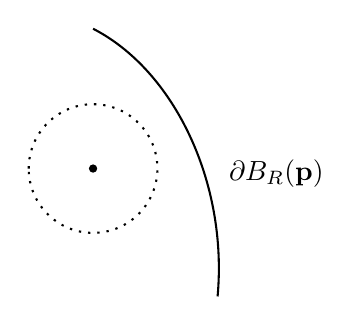
\begin{tikzpicture}[x=0.75pt,y=0.75pt,yscale=-1,xscale=1]
            %uncomment if require: \path (0,138); %set diagram left start at 0, and has height of 138

            %Curve Lines [id:da3646608908276512] 
            \draw    (253,4.63) .. controls (292,24.63) and (318,78.63) .. (313,133.63) ;
            %Shape: Circle [id:dp25903533863346984] 
            \draw  [dash pattern={on 0.84pt off 2.51pt}] (222,72) .. controls (222,54.88) and (235.88,41) .. (253,41) .. controls (270.12,41) and (284,54.88) .. (284,72) .. controls (284,89.12) and (270.12,103) .. (253,103) .. controls (235.88,103) and (222,89.12) .. (222,72) -- cycle ;
            %Shape: Circle [id:dp6902212722781198] 
            \draw  [draw opacity=0][fill={rgb, 255:red, 0; green, 0; blue, 0 } ,fill opacity=1 ] (251,72) .. controls (251,70.9) and (251.9,70) .. (253,70) .. controls (254.1,70) and (255,70.9) .. (255,72) .. controls (255,73.1) and (254.1,74) .. (253,74) .. controls (251.9,74) and (251,73.1) .. (251,72) -- cycle ;

            % Text Node
            \draw (317,66.4) node [anchor=north west][inner sep=0.75pt]    {$\partial B_{R}(\mathbf{p})$};
            % Text Node
            \draw (255,73.4) node [anchor=north west][inner sep=0.75pt]    {$\x$};

        \end{tikzpicture}

    \end{figure}
    \FloatBarrier

    possiamo passare al limite sotto il segno di integrale perché il denominatore non si annulla mai, e in particolare risulta $u\in C^{\infty }(B_{R}(\mathbf{p}))$.\footnote{"Why are we still here? Just to suffer?".}

    \textbf{Caso con }$G\in C([0,2\pi])$, solamente continua. La \eqref{eq:poisson-cerchio-dim} definisce $u\in C^{\infty }(B_{R}(\mathbf{p}))$ e armonica in $B_{R}(\mathbf{p})$. L'unica cosa un po' delicata sono le condizioni al bordo, che comunque si possono verificare.

\end{dimostrazione}

\LezioneS{22/03/2021}

Possiamo generalizzare la \eqref{eq:poisson-cerchio} per un numero generico $n$ di dimensioni
\begin{equation*}
    u(\x) =\frac{R^{2} -| \x -\mathbf{p}| ^{2}}{w_{n} R}\int _{\partial B_{R}(\mathbf{p})}\frac{g(\sigg)}{| \x -\sigg| ^{n}} \dsig
\end{equation*}
con $\displaystyle u\in C^{\infty }(B_{R}(\mathbf{p})) \cap C\left(\overline{B_{R}}(\mathbf{p})\right)$.
\section{Soluzione fondamentale per l'operatore di Laplace}

Come abbiamo trovato e costruito una soluzione fondamentale per l'operatore del calore, cerchiamo una soluzione con proprietà simili per l'operatore di Laplace: questa soluzione fondamentale, armonica in tutto $\displaystyle \mathbb{R}^{n}$ tranne che in un punto, ci servirà per costruire una formula di rappresentazione per la soluzione del problema di Dirichlet che coinvolge dei potenziali.

Sia $\displaystyle u=u(\x)$ armonica in $\displaystyle \mathbb{R}^{n}$ e sia $M$ una matrice di rotazione, cioè tale che
\begin{equation*}
    M^{T} =M^{-1} \ \ \land \ \ \mathrm{det} M=1
\end{equation*}
Iniziamo osservando che, definita $\displaystyle D^{2} u$ l'Hessiana di $u$, possiamo scrivere
\begin{equation*}
    \Delta u=\mathrm{Tr} D^{2} u
\end{equation*}
Definiamo $v(\x) =u(M\x)$, allora
\begin{equation*}
    D^{2} v(\x) =M^{T} D^{2} u(M\x) M
\end{equation*}
inoltre
\begin{align*}
    \Delta v(\x) & =\mathrm{Tr}\left[ M^{T} D^{2} u(M\x) M\right] &                                        \\
                 & =\mathrm{Tr} D^{2} u(M\x)                      & M\ \text{ortogonale non varia traccia} \\
                 & =\Delta u(M\x) =0                              &
\end{align*}
$v$ è ancora armonica: \textbf{il Laplaciano commuta con le rotazioni} e dunque $\Delta $ è invariante per rotazioni. Si dimostra facilmente che $\Delta $ \textbf{è anche invariante per traslazione}: se $u(\x)$ è armonica, $v(\x) =u(\x-\y)$, per ogni $\y$ fissato, è armonica.

Per l'operatore del calore la soluzione fondamentale (in $n=3$) era
\begin{equation*}
    \Gamma _{D}(\x,t) =\frac{1}{(4\pi Dt)^{3/2}}\exp\left\{-\frac{\textcolor[rgb]{0.82,0.01,0.11}{|\x|^{2}}}{4D\textcolor[rgb]{0.82,0.01,0.11}{t}}\right\}
\end{equation*}
Il blocco $\displaystyle \textcolor[rgb]{1,0,0}{\frac{|\x|^{2}}{t}}$ è invariante per dilatazioni paraboliche della forma
\begin{align*}
    \x & \longmapsto a\x     \\
    t  & \longmapsto a^{2} t
\end{align*}
Dove il tempo \textit{conta} come il quadrato dello spazio: questo non è altro che il riflesso dell'operatore del calore stesso, dove una derivata temporale \textit{compensava} una derivata seconda spaziale
\begin{equation*}
    u_{t} -Du_{xx} =0
\end{equation*}
Per analogia ci aspettiamo che, essendo l'operatore di Laplace invariante per rotazioni, anche la soluzione fondamentale per l'operatore Laplaciano sia invariante per rotazioni. Cerchiamo quindi una soluzione della forma
\begin{equation*}
    u=u(|\x|)
\end{equation*}
Poniamo $\displaystyle r=|\x| $ e cerchiamo $\displaystyle u=u(r)$ tale che
\begin{equation*}
    \Delta u=0\ \text{in} \ \mathbb{R}^{n} \setminus \{0\},\ n=2,3
\end{equation*}
In $0$ non può essere armonica perché non è derivabile. Dato che la soluzione è radiale conviene passare alle coordinate polari
\begin{itemize}
    \item $n=2$
          \begin{equation*}
              \Delta _{\text{polare}} u(r) =u_{rr} +\frac{1}{r} u_{r} +\cancel{\frac{1}{r^{2}} u_{\vartheta \vartheta }} =0
          \end{equation*}

          Risolvendo separando le variabili
          \begin{align*}
              \frac{u_{rr}}{u_{r}} & =-\frac{1}{r}  \\
              \log| u_{r}|         & =-\log r+c_{1}
          \end{align*}

          Definendo $\displaystyle k=e^{c_{1}}  >0$
          \begin{equation*}
              | u_{r}| =k\frac{1}{r}
          \end{equation*}

          Liberandoci infine del modulo ($\displaystyle k\in \mathbb{R}$)
          \begin{equation*}
              u_{r} =k\frac{1}{r}
          \end{equation*}

          Otteniamo la soluzione
          \begin{equation*}
              \boxed{u(r) =k\log r+k_{1}} \ \ (r\neq 0)
          \end{equation*}
    \item $n=3$
          \begin{align*}
              \Delta _{\text{sferico}} u(r) =u_{rr} +\frac{2}{r} u_{r} & =0    \\
              (ru)_{rr}                                                & =0    \\
              ru                                                       & =Ar+B
          \end{align*}

          Che dà come soluzione
          \begin{equation*}
              \boxed{u(r) =A+\frac{B}{r}} \ \ (r\neq 0)
          \end{equation*}
\end{itemize}

Per ottenere la soluzione fondamentale devo scegliere le costanti in modo tale che\footnote{Il procedimento per la scelta delle costanti sarà svolto nella parte di analisi funzionale, nella sezione \vref{sec:controesempio-derivata-debole-classica}.}
\begin{equation*}
    -\Delta u=\delta _{n} \ \text{in} \ \mathbb{R}^{n}
\end{equation*}
Da cui ricaviamo la \textbf{soluzione fondamentale}
\begin{equation}
    \boxed{\Phi (\x) =
        \begin{cases}
            -\frac{1}{2\pi }\log|\x| & n=2 \\
            \frac{1}{4\pi |\x| }     & n=3
        \end{cases}}
\end{equation}
$\displaystyle \Phi $ è definita per $\displaystyle x\neq 0$ e ha significato fisico. Se $n=3$, $\displaystyle 4\pi \Phi $ rappresenta il potenziale elettrostatico generato da una carica posta nell'origine che si annulla all'infinito. Se $n=2$, $\displaystyle 2\pi \Phi $ rappresenta il potenziale generato da una carica di densità totale $1$, distribuita lungo l'asse $\displaystyle x_{3}$.

Se la carica è posta in un punto $\y$ fissato possiamo sfruttare l'invarianza per traslazione
\begin{equation*}
    \Delta _{\x} \Phi (\x-\y) =-\delta _{\y}
\end{equation*}
E per simmetria, con $\x$ fissato
\begin{equation*}
    \Delta _{\y} \Phi (\x-\y) =-\delta _{\x}
\end{equation*}
Generalizzando per dimensione $n >3$ la soluzione fondamentale è
\begin{equation*}
    \Phi (\x) =\frac{1}{(n-2) w_{n}}\frac{1}{|\x| ^{n-2}}
\end{equation*}
\section{Il potenziale Newtoniano}

Torniamo in dimensione $n=3$. Supponiamo che $\displaystyle \frac{1}{4\pi } f(\y)$ rappresenti la densità di una carica localizzata all'interno di un compatto di $\displaystyle \mathbb{R}^{3}$. Il potenziale in $x$ generato dalla carica presente in un piccolo volumetto $\dy$, centrata in $y$, è dato da
\begin{equation*}
    \Phi (\x-\y) f(\y) \dyy
\end{equation*}
Il potenziale totale si ottiene sommando tutti i contributi
\begin{equation}
    \mathcal{N}_{f}(\x) =\int _{\mathbb{R}^{3}} \Phi (\x-\y) f(\y) \dyy=\frac{1}{4\pi }\int _{\mathbb{R}^{3}}\frac{f(\y)}{|\x-\y| } \dyy=(\Phi \ast f)(\x)
\end{equation}
Questo potenziale è detto \textbf{potenziale Newtoniano} di $f$. Formalmente, nel senso delle distribuzioni e sotto opportune ipotesi per $f$\footnote{Per $x$ fissato $\frac{1}{|\x-\y| } \in L^{1}(B(\zer))$, quindi dovrò controllare solo il comportamento di $f(\y)$.}:
\begin{equation*}
    -\Delta \mathcal{N}_{f}(\x) =(-\Delta \Phi \ast f)(\x) =(\delta _{3} \ast f)(\x) =\int _{\mathbb{R}^{3}} \delta _{3}(\x-\y) f(\y) \dyy=f(\x)
\end{equation*}
Formalizziamo in un teorema.
\begin{theorem}
    Sia $\displaystyle f\in C^{2}\left(\mathbb{R}^{3}\right)$ a supporto compatto. Allora $\displaystyle \mathcal{N}_{f} \in C^{2}\left(\mathbb{R}^{3}\right)$ ed è l'unica soluzione dell'equazione di Poisson
    \begin{equation*}
        -\Delta u=f\ \text{in} \ \mathbb{R}^{3}
    \end{equation*}
    \textbf{che si annulla all'infinito}.
\end{theorem}
In generale anche $\mathcal{N}_{f}+c$ è soluzione, ma questa è quella che si annulla all'infinito.
\begin{nb}
    Per $n=2$ il potenziale Newtoniano si chiama potenziale logaritmico
    \begin{equation}
        \mathcal{L}_{f}(\x) =-\frac{1}{2\pi }\int _{\mathbb{R}^{2}}\log|\x-\y| f(\y) \dyy
    \end{equation}
    e vale un risultato simile: se $\displaystyle f\in C^{2}(\mathbb{R}^{2})$, allora $\displaystyle \mathcal{L}_{f} \in C^{2}(\mathbb{R}^{2})$ ed è l'unica soluzione di
    \begin{equation*}
        -\Delta u=f\ \text{in} \ \mathbb{R}^{2}
    \end{equation*}
    con andamento asintotico
    \begin{equation*}
        u(\x) =-\frac{M}{2\pi }\log|\x| +o\left(\frac{1}{|\x| }\right),\quad |\x| \rightarrow +\infty
    \end{equation*}
    Dove $M$ è la carica totale
    \begin{equation*}
        M=\int _{\mathbb{R}^{2}} f(\y) \dyy
    \end{equation*}
\end{nb}
\section{La funzione di Green}
Abbiamo considerato tutto $\mathbb{R} ^{n} $, ma se invece consideriamo una regione finita dobbiamo tenere conto del bordo. Richiediamo che sia regolare in modo da considerare le derivate normali.
\begin{theorem}
    Sia $\displaystyle \Omega \subset \mathbb{R}^{3}$ un \textbf{dominio limitato e regolare}, sia $\displaystyle u\in C^{2}(\overline{\Omega }$). Allora la soluzione del problema di Dirichlet $\Delta u=f$ con $u=g$ al bordo è:
    \begin{equation*}
        u(\x)=-\underbrace{\int _{\Omega } \Phi (\x-\y) f(\y) \dyy}_{\substack{\text{potenziale Newtoniano}\\\text{di } f=\Delta u}}
        +\underbrace{\int _{\partial \Omega } \Phi (\x-\sigg) \partial _{\nuu} u(\sigg) \dsig }_{\substack{\text{potenziale di strato semplice}\\\text{con densità }\partial _{\nuu} u}}
        -\underbrace{\int _{\partial \Omega } u(\sigg) \partial _{\nuu} \Phi (\x-\sigg) \dsig }_{ \substack{\text{potenziale di doppio strato}\\\text{con momento }\mu}}
    \end{equation*}
\end{theorem}
In pratica, ogni funzione regolare $u$ può essere scritta come somma di un potenziale di volume (Newtoniano) con densità $\displaystyle -\Delta u$, di un potenziale di strato semplice causato da una densità di cariche $\displaystyle \partial _{\nuu} u$ superficiali sul bordo $\displaystyle \partial \Omega $ e da un potenziale di doppio strato generato da dei dipoli elettrici con momento $\mu $.

Vediamo la dimostrazione del teorema.
\begin{dimostrazione}
    Ricordiamo innanzitutto l'identità di Green con $\displaystyle u,v\in C^{2}(\overline{\Omega })$
    \begin{equation*}
        \int _{\Omega }(v\Delta u-u\Delta v) \dxx =\int _{\partial \Omega }(v\partial _{\nuu} u-u\partial _{\nuu} v) \dsig
    \end{equation*}
    Applichiamo l'identità di Green utilizzando come funzione $u$ la stessa dell'enunciato del teorema. Per la funzione $v$ dobbiamo trovare un'alternativa, infatti, con $\x$ fissato
    \begin{equation*}
        v(\y) =\Phi (\x -\y) =\frac{1}{4\pi }\frac{1}{| \x -\y| } \notin C^{2}(\Omega)
    \end{equation*}
    Con $\displaystyle \Omega $ dominio limitato, definisco
    \begin{equation*}
        \Omega _{\varepsilon } =\Omega \setminus \overline{B}_{\varepsilon }(\x)
    \end{equation*}
    \begin{figure}[H]
        \centering
        \tikzset{every picture/.style={line width=0.75pt}} %set default line width to 0.75pt        

        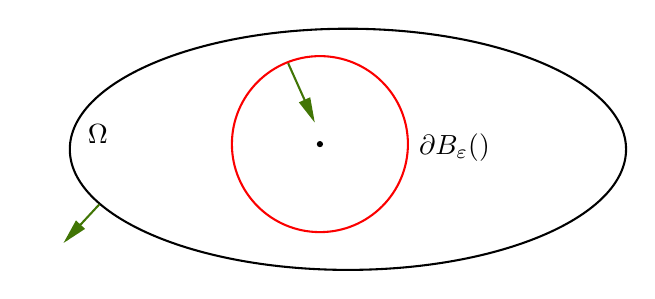
\begin{tikzpicture}[x=0.75pt,y=0.75pt,yscale=-1,xscale=1]
            %uncomment if require: \path (0,141); %set diagram left start at 0, and has height of 141

            %Shape: Ellipse [id:dp8534708959725636] 
            \draw   (100,73.1) .. controls (100,41.01) and (159.99,15) .. (234,15) .. controls (308.01,15) and (368,41.01) .. (368,73.1) .. controls (368,105.19) and (308.01,131.2) .. (234,131.2) .. controls (159.99,131.2) and (100,105.19) .. (100,73.1) -- cycle ;
            %Shape: Ellipse [id:dp5474821128070129] 
            \draw  [draw opacity=0][fill={rgb, 255:red, 0; green, 0; blue, 0 }  ,fill opacity=1 ][line width=3]  (222,70.6) .. controls (222,69.77) and (221.33,69.1) .. (220.5,69.1) .. controls (219.67,69.1) and (219,69.77) .. (219,70.6) .. controls (219,71.43) and (219.67,72.1) .. (220.5,72.1) .. controls (221.33,72.1) and (222,71.43) .. (222,70.6) -- cycle ;
            %Shape: Ellipse [id:dp9123452672283427] 
            \draw  [color={rgb, 255:red, 251; green, 0; blue, 0 }  ,draw opacity=1 ] (178.1,70.6) .. controls (178.1,47.18) and (197.08,28.2) .. (220.5,28.2) .. controls (243.92,28.2) and (262.9,47.18) .. (262.9,70.6) .. controls (262.9,94.02) and (243.92,113) .. (220.5,113) .. controls (197.08,113) and (178.1,94.02) .. (178.1,70.6) -- cycle ;
            %Straight Lines [id:da4961016004934615] 
            \draw [color={rgb, 255:red, 65; green, 117; blue, 5 }  ,draw opacity=1 ]   (114.2,99.65) -- (98.36,116.74) ;
            \draw [shift={(97,118.2)}, rotate = 312.83000000000004] [fill={rgb, 255:red, 65; green, 117; blue, 5 }  ,fill opacity=1 ][line width=0.08]  [draw opacity=0] (12,-3) -- (0,0) -- (12,3) -- cycle    ;
            %Straight Lines [id:da5401738716118851] 
            \draw [color={rgb, 255:red, 65; green, 117; blue, 5 }  ,draw opacity=1 ]   (205.2,31.65) -- (217.18,58.38) ;
            \draw [shift={(218,60.2)}, rotate = 245.85] [fill={rgb, 255:red, 65; green, 117; blue, 5 }  ,fill opacity=1 ][line width=0.08]  [draw opacity=0] (12,-3) -- (0,0) -- (12,3) -- cycle    ;

            % Text Node
            \draw (107.2,59.8) node [anchor=north west][inner sep=0.75pt]    {$\Omega $};
            % Text Node
            \draw (266.83,64) node [anchor=north west][inner sep=0.75pt]  [font=\normalsize]  {$\partial B_{\varepsilon }(\x)$};
            % Text Node
            \draw (80.2,104.8) node [anchor=north west][inner sep=0.75pt]  [font=\normalsize,color={rgb, 255:red, 65; green, 117; blue, 5 }  ,opacity=1 ]  {$\nuu$};
            % Text Node
            \draw (196.2,40.8) node [anchor=north west][inner sep=0.75pt]  [font=\normalsize,color={rgb, 255:red, 65; green, 117; blue, 5 }  ,opacity=1 ]  {$\nuu$};
            % Text Node
            \draw (221,74) node [anchor=north west][inner sep=0.75pt]    {$\x$};

        \end{tikzpicture}
    \end{figure}
    \FloatBarrier

    In $\displaystyle \Omega _{\varepsilon }$, $\displaystyle v(\y) \in C^{2}\left(\overline{\Omega _{\varepsilon }}\right)$ e inoltre $\displaystyle \Delta v=0$ in $\displaystyle \Omega _{\varepsilon }$.

    Si trova tutto a partire dall'identità di Green con questa scelta di $u$ e $v$ si elide il termine $\displaystyle u\Delta v=0$.
    \begin{equation*}
        \frac{1}{4\pi }\underbrace{\int _{\Omega _{\varepsilon }}\frac{1}{| \x -\y| } f(\y) \dyy}_{(1)} =\frac{1}{4\pi }\underbrace{\int _{\partial \Omega _{\varepsilon }}\frac{1}{| \x -\sigg| } \partial _{\nuu} u(\sigg) \dsig}_{(2)} -\frac{1}{4\pi }\underbrace{\int _{\partial \Omega _{\varepsilon }} u(\sigg) \partial _{\nuu}\frac{1}{| \x -\sigg| } \dsig}_{(3)}
    \end{equation*}
    Inoltre
    \begin{equation*}
        \partial \Omega _{\varepsilon } =\partial \Omega \cup \partial B_{\varepsilon }(\x)
    \end{equation*}
    E su $\displaystyle \partial B_{\varepsilon }(\x)$
    \begin{equation*}
        \nuu(\sigg) =\frac{\x -\sigg}{| \x -\sigg| } =\frac{\x -\sigg}{\varepsilon }
    \end{equation*}
    Studiamo come si comporta ciascun termine dell'identità al limite per $\displaystyle \varepsilon \rightarrow 0$
    \begin{itemize}
        \item \textbf{Termine 1}

              \begin{equation*}
                  (1) =\int _{\Omega _{\varepsilon }}\frac{1}{| \x -\y| } f(\y) \dyy =\int _{\Omega }\underbrace{\chi _{\Omega _{\varepsilon }}(\y)\frac{f(\y)}{| \x -\y| }}_{g_{\varepsilon }(\y)} \dyy
              \end{equation*}

              Con

              \begin{equation*}
                  | g_{\varepsilon }(\y)| \leq \max\frac{| f| }{| \x -\y| }
              \end{equation*}

              Posso usare il teorema di convergenza dominata e passare al limite sotto il segno di integrale, il primo termine tende a

              \begin{equation*}
                  (1)\rightarrow \int _{\Omega }\frac{1}{| \x -\y| } f(\y) \dyy
              \end{equation*}

              A meno del coefficiente, questo è diventato il potenziale Newtoniano.
        \item \textbf{Termine 2}

              \begin{equation*}
                  \int _{\partial \Omega _{\varepsilon }}\frac{\partial _{\nuu} u(\sigg)}{| \x -\sigg| } \dsig =\left(\int _{\partial \Omega } +\int _{\partial B_{\varepsilon }(\x)}\right)\frac{\partial _{\nuu} u(\sigg)}{| \x -\sigg| } \dsig
              \end{equation*}

              Di questi, quello sul bordo della palla andrà a zero.

              Ricordando che

              \begin{equation*}
                  | \partial _{\nuu} u(\sigg)| =| \nabla u(\sigg) \cdotp \nuu| \leq \max| \nabla u|
              \end{equation*}

              maggioriamo
              \begin{align*}
                  \left| \int _{\partial B_{\varepsilon }(\x)}\frac{\partial _{\nuu} u(\sigg)}{| \x -\sigg| } \dsig\right| & \leq \int _{\partial B_{\varepsilon }(\x)}\frac{| \partial _{\nuu} u(\sigg)| }{\underbrace{| \x -\sigg| }_{=\varepsilon }} \dsig \\
                                                                                                                           & \leq \frac{1}{\varepsilon }\int _{\partial B_{\varepsilon }(\x)}\max| \nabla u| \dsig                                            \\
                                                                                                                           & =\frac{\max| \nabla u| }{\varepsilon }\int _{\partial B_{\varepsilon }(\x)} \dsig                                                     \\
                                                                                                                           & =\frac{\max| \nabla u| }{\varepsilon } \cdotp 4\pi \varepsilon ^{2}\rightarrow 0
              \end{align*}

              L'altro non dipende da $\displaystyle \varepsilon $ quindi rimane così.
              \begin{equation*}
                  (2)\rightarrow \int _{\partial \Omega }\frac{\partial _{\nuu} u(\sigg)}{| \x -\sigg| } \dsig
              \end{equation*}

              A meno del coefficiente, questo è diventato il potenziale di strato semplice.
        \item \textbf{Termine 3}

              Da qui spunteranno sia il potenziale di doppio strato, che la $u$ stessa.

              \begin{equation*}
                  (3) =\int _{\partial \Omega _{\varepsilon }} u(\sigg) \partial _{\nuu}\frac{1}{| \x -\sigg| } \dsig =\left(\int _{\partial \Omega } +\int _{\partial B_{\varepsilon }(\x)}\right) u(\sigg) \partial _{\nuu}\frac{1}{| \x -\sigg| } \dsig
              \end{equation*}

              L'integrale su $\displaystyle \partial \Omega $ è già il potenziale di doppio strato, ci manca da far vedere che l'altro tende a $u$, a meno del coefficiente. Calcolo la derivata normale su $\displaystyle \partial B_{\varepsilon }(\x)$ con la regola della catena
              \begin{equation*}
                  \nabla _{\sigg}\frac{1}{| \x -\sigg| } =-\frac{1}{| \x -\sigg| ^{2}} \cdotp \frac{\x -\sigg}{| \x -\sigg| }(-1) =\frac{\x -\sigg}{| \x -\sigg| ^{3}} =\frac{\x -\sigg}{\varepsilon ^{3}}
              \end{equation*}

              quindi
              \begin{equation*}
                  \partial _{\nuu}\frac{1}{| \x -\sigg| } =\nabla \frac{1}{| \x -\sigg| } \cdotp \nuu =\frac{\x -\sigg}{\varepsilon ^{3}} \cdotp \frac{\x -\sigg}{\varepsilon } =\frac{1}{\varepsilon ^{2}}
              \end{equation*}

              Da cui
              \begin{align*}
                  \int _{\partial B_{\varepsilon }(\x)} u(\sigg) \partial _{\nuu}\frac{1}{| \x -\sigg| } \dsig & =\frac{1}{\varepsilon ^{2}}\int _{\partial B_{\varepsilon }(\x)} u(\sigg) \dsig                                                                                                                   \\
                                                                                                               & =\frac{4\pi \varepsilon ^{2}}{\varepsilon ^{2}} \cdotp \underbrace{\frac{1}{4\pi \varepsilon ^{2}}\int _{\partial B_{\varepsilon }(\x)} u(\sigg) \dsig}_{\rightarrow u(\x)}\rightarrow 4\pi u(\x)
              \end{align*}

              quindi
              \begin{equation*}
                  (3)\rightarrow \int _{\partial \Omega } u(\sigg) \partial _{\nuu}\frac{1}{| \x -\sigg| } \dsig +4\pi u(\x)
              \end{equation*}

              Riassemblando i vari pezzi si ottiene la tesi.
    \end{itemize}
\end{dimostrazione}

\LezioneS{23/03/2021}
\section{Funzione di Green e formula di rappresentazione}

Ci proponiamo di ottenere una formula di rappresentazione \textbf{in funzione dei dati} del seguente problema di Dirichlet
\begin{equation}
    \begin{cases}
        -\Delta u=f & \text{in} \ \Omega          \\
        u=\varphi , & \text{su} \ \partial \Omega
    \end{cases}
    \label{eq:sol-green-pb-dirichlet}
\end{equation}
Richiamiamo la formula della lezione scorsa
\begin{equation}
    u(\x) =-\int _{\Omega } \Phi (\x-\y) \Delta u(\y) \dyy+\int _{\partial \Omega } \Phi (\x-\sigg) \underbrace{\partial _{\nuu} u(\sigg)}_{?} \dsig -\int _{\partial \Omega } \partial _{\nuu} \Phi (\x-\sigg) u(\sigg) \dsig
    \label{eq:richiamo-formula-green}
\end{equation}
Conosciamo $\Delta u$, essendo uguale a $f$ come dato del problema, e conosciamo anche $u(\sigg)$ sul bordo, essendo uguale al dato $g$, ma non sappiamo nulla del termine $\partial _{\nuu} u(\sigg)$. L'idea è di andare a cercare una funzione $G$ tale che \textit{si annulli sul bordo}, così che il termine centrale si annulli. Sia $g(\x,\y)$ la soluzione di un certo problema
\begin{equation}
    \begin{cases}
        -\Delta _{\y} g=0,           & \text{in} \ \Omega          \\
        g(\x,\sigg) =\Phi (\x-\sigg) & \text{su} \ \partial \Omega
    \end{cases}
    \label{eq:sol-green-pb-unico}
\end{equation}
Basta definire la seguente \textbf{funzione di Green per l'operatore di Laplace in} $\Omega $
\begin{equation*}
    \boxed{G(\x,\y) =\Phi (\x-\y) -g(\x,\y)}
\end{equation*}
ottenendo, siccome il laplaciano di $g$ è nullo,
\begin{equation*}
    \begin{cases}
        -\Delta _{\y} G(\x,\y) =\delta (\x) & \text{in} \ \Omega          \\
        G(\x,\sigg) =0                      & \text{su} \ \partial \Omega
    \end{cases}
\end{equation*}
Dall'identità di Green \eqref{eq:id-green} applicata a $u$ e
\begin{equation}
    v(\y) =g(\x,\y) \ \text{con} \ x\ \text{fissato}
    \label{eq:sol-green-v-g}
\end{equation}
da cui
\begin{align*}
    \int _{\Omega }(v\Delta u-u\Delta v) \dxx & =\cancel{-\int _{\Omega } \nabla v\cdotp \nabla u} +\int _{\partial \Omega } v\partial _{\nuu} u-\left(\cancel{-\int _{\Omega } \nabla u\cdotp \nabla v} +\int _{\partial \Omega } u\partial _{\nuu} v\right) \\
                                              & =\int _{\partial \Omega }(v\partial _{\nuu} u-u\partial _{\nuu} v) \dsig
\end{align*}
sostituiamo le relazioni \eqref{eq:sol-green-pb-dirichlet}, \eqref{eq:sol-green-pb-unico}, \eqref{eq:sol-green-v-g} e ricordiamo che $\Delta v=\Delta _{y} g=0$
\begin{align*}
    -\int _{\Omega } \underbrace{g(\x,\y)}_{v} \underbrace{f(\y)}_{\Delta u} \dyy & =\int _{\partial \Omega } \underbrace{\Phi (\x-\sigg)}_{v} \partial _{\nuu} u\dsig -\int _{\partial \Omega } \underbrace{\varphi (\sigg)}_{u} \partial _{\nuu} \underbrace{g(\x,\sigg)}_{v} \dsig \\
    0                                                                             & =\int _{\Omega } g(\x,\y) f(\y) \dyy+\int _{\partial \Omega } \Phi (\x-\sigg) \partial _{\nuu} u\dsig -\int _{\partial \Omega } \varphi (\sigg) \partial _{\nuu} g(\x,\sigg) \dsig
\end{align*}
facendo la differenza tra \eqref{eq:richiamo-formula-green} e questa scompare il termine con la derivata normale sul bordo
\begin{equation*}
    u(\x) =\int _{\Omega }\underbrace{[ \Phi (\x-\y) -g(\x,\y)]}_{G(\x,\y)} f(\y) \dyy+0-\int _{\partial \Omega } \varphi (\sigg) \partial_{\nuu}\underbrace{[ \Phi (\x-\sigg) -g(\x,\sigg)]}_{G(\x,\sigg)} \dsig
\end{equation*}
cioè abbiamo ottenuto la \textbf{formula di rappresentazione di Green}\footnote{Si noti che anche se $G$ è nulla sul bordo, non è detto che la sua derivata normale sia nulla, è facile rendersene conto pensando al caso unidimensionale.}
\begin{equation*}
    \boxed{u(\x) =\int _{\Omega } G(\x,\y) f(\y) \dyy-\int _{\partial \Omega } \varphi (\sigg) \partial_{\nuu} G(\x,\sigg) \dsig }
\end{equation*}
questa formula è utile perché per risolvere qualunque problema di Dirichlet per qualunque coppia di dati $f,\varphi $ è sufficiente risolvere un solo problema, il \eqref{eq:sol-green-pb-unico}, da cui si costruisce la $G$ e si trova $u$.